% Options for packages loaded elsewhere
\PassOptionsToPackage{unicode}{hyperref}
\PassOptionsToPackage{hyphens}{url}
%
\documentclass[
]{article}
\usepackage{lmodern}
\usepackage{amssymb,amsmath}
\usepackage{ifxetex,ifluatex}
\ifnum 0\ifxetex 1\fi\ifluatex 1\fi=0 % if pdftex
  \usepackage[T1]{fontenc}
  \usepackage[utf8]{inputenc}
  \usepackage{textcomp} % provide euro and other symbols
\else % if luatex or xetex
  \usepackage{unicode-math}
  \defaultfontfeatures{Scale=MatchLowercase}
  \defaultfontfeatures[\rmfamily]{Ligatures=TeX,Scale=1}
\fi
% Use upquote if available, for straight quotes in verbatim environments
\IfFileExists{upquote.sty}{\usepackage{upquote}}{}
\IfFileExists{microtype.sty}{% use microtype if available
  \usepackage[]{microtype}
  \UseMicrotypeSet[protrusion]{basicmath} % disable protrusion for tt fonts
}{}
\makeatletter
\@ifundefined{KOMAClassName}{% if non-KOMA class
  \IfFileExists{parskip.sty}{%
    \usepackage{parskip}
  }{% else
    \setlength{\parindent}{0pt}
    \setlength{\parskip}{6pt plus 2pt minus 1pt}}
}{% if KOMA class
  \KOMAoptions{parskip=half}}
\makeatother
\usepackage{xcolor}
\IfFileExists{xurl.sty}{\usepackage{xurl}}{} % add URL line breaks if available
\IfFileExists{bookmark.sty}{\usepackage{bookmark}}{\usepackage{hyperref}}
\hypersetup{
  hidelinks,
  pdfcreator={LaTeX via pandoc}}
\urlstyle{same} % disable monospaced font for URLs
\usepackage[margin=1in]{geometry}
\usepackage{graphicx,grffile}
\makeatletter
\def\maxwidth{\ifdim\Gin@nat@width>\linewidth\linewidth\else\Gin@nat@width\fi}
\def\maxheight{\ifdim\Gin@nat@height>\textheight\textheight\else\Gin@nat@height\fi}
\makeatother
% Scale images if necessary, so that they will not overflow the page
% margins by default, and it is still possible to overwrite the defaults
% using explicit options in \includegraphics[width, height, ...]{}
\setkeys{Gin}{width=\maxwidth,height=\maxheight,keepaspectratio}
% Set default figure placement to htbp
\makeatletter
\def\fps@figure{htbp}
\makeatother
\setlength{\emergencystretch}{3em} % prevent overfull lines
\providecommand{\tightlist}{%
  \setlength{\itemsep}{0pt}\setlength{\parskip}{0pt}}
\setcounter{secnumdepth}{-\maxdimen} % remove section numbering
%latex header to wrap code lines in .pdf

\usepackage{fvextra}
\DefineVerbatimEnvironment{Highlighting}{Verbatim}{breaklines,commandchars=\\\{\}}

% To keep the figure from floating around
% All figures should be forced in-place via the [H]ERE float specification.
\usepackage{float}
\floatplacement{figure}{H}
%\floatplacement{figure}{!htbp}

\date{}

\begin{document}

\hypertarget{report-of-the-fit}{%
\section{Report of the fit}\label{report-of-the-fit}}

\hypertarget{fit-summary}{%
\subsection{Fit summary}\label{fit-summary}}

Description: PV19 version x. Initial fit parameters from a previous fit
with ceres on replica zero. Negative g2 as stating parameters, the chi2
of replica 0 without minimisation with this fitconfig file was
1.10947.\\
Minimiser: minuit\\
Random seed: 1234\\
Maximum values allowed for \(q_T / Q\): 0.2\\
Cut on the error function: 4\\
Parameterisation: PV19x\\
Explicit formula:

\[f_{\rm NP}(x,\zeta, b_T)= \Biggl(
\frac{1-\lambda}{1 + g_1(x) b_T^2/4} + \lambda \exp \left(-g_{1B}(x) b_T^2 / 4 \right)\Biggr) \exp\left[- g_2 \log\left(\frac{\zeta}{Q_0^2}\right) b_T^2/4 - g_{2B} \log\left(\frac{\zeta}{Q_0^2}\right) b_T^4/4 \right]\]\[g_1(x) = \frac{N_1}{x\sigma} \exp\left[ - \frac{\ln^2\left(\frac{x}{\alpha}\right)}{2 \sigma^2} \right]\]\[g_{1B}(x) = \frac{N_{1B}}{x\sigma_B} \exp\left[ - \frac{\ln^2\left(\frac{x}{\alpha_B}\right)}{2 \sigma_B^2} \right]\]\[Q_0^2 = 1\;{\rm GeV}^2\]
\(t_0\) prescription: True

\begin{table}[h]

\centering

\begin{tabular}{|c|c|c|c|c|c|c|c|c|} \hline

\textbf{\(g_2\)} & \textbf{\(N_1\)} & \textbf{\(\alpha\)} & \textbf{\(\sigma\)} & \textbf{\(\lambda\)} & \textbf{\(N_{1B}\)} & \textbf{\(\alpha_B\)} & \textbf{\(\sigma_B\)} & \textbf{\(g_{2B}\)} \\ \hline

-0.005144 & 0.68535248 & 0.21943481 & 0.3329461 & 0.66627605 & 0.0387879 & 0.075758463 & 0.34845635 & 0.019224141 \\ \hline

\end{tabular}

\caption{}

\end{table}

\hypertarget{theory-summary}{%
\subsection{Theory summary}\label{theory-summary}}

Collinear PDF set: MMHT2014nnlo68cl member 0\\
Collinear FF set: DSS14\_NLO\_PiSum member 0\\
\(b^*\) prescription: bstarmin\\
Perturbative order: NNLLp\\
Initial parameters fluctuations: True\\
Reference value of the fine-structure constant:
\(\alpha(Q = 91.1876\;{\rm GeV}) = 0.00776578395589\) (running True)

\hypertarget{global-statistical-estimators}{%
\subsection{Global statistical
estimators}\label{global-statistical-estimators}}

\(N_{rep}\) = 166\\
\(\chi_{0}^2\) = 1.1092\\
\(\chi_{mean}^2\) = 1.1253\\
\(\langle\chi^2\rangle \pm \sigma_{\chi^2}\) = 1.1393 \(\pm\) 0.018\\
\(\langle E \rangle \pm \sigma_{E}\) = 2.124 \(\pm\) 0.1813

\hypertarget{parameters}{%
\subsection{Parameters}\label{parameters}}

\begin{table}[h]

\centering

\begin{tabular}{|c|c|c|c|} \hline

\textbf{Parameter} & \textbf{Central replica} & \textbf{Average over
replicas} & \textbf{Fixed} \\ \hline

\(g_2\) & -0.0053704255 & -0.00704821 \(\pm\)
0.01063546 & False \\ \hline
\(N_1\) & 0.65700739 & 0.81060207 \(\pm\) 0.42482512 & False \\ \hline
\(\alpha\) & 0.2182943 & 0.22897105 \(\pm\) 0.02058738 & False \\ \hline
\(\sigma\) & 0.33326516 & 0.30438571 \(\pm\)
0.08461941 & False \\ \hline
\(\lambda\) & 0.65465646 & 0.65049177 \(\pm\)
0.08422013 & False \\ \hline
\(N_{1B}\) & 0.039906833 & 13.19571078 \(\pm\)
168.90703882 & False \\ \hline
\(\alpha_B\) & 0.075999739 & 0.08057839 \(\pm\)
0.02231829 & False \\ \hline
\(\sigma_B\) & 0.35204268 & 0.32460359 \(\pm\)
0.11180911 & False \\ \hline
\(g_{2B}\) & 0.018927351 & 0.01954714 \(\pm\)
0.00404642 & False \\ \hline

\end{tabular}

\caption{}

\end{table}

\begin{figure}
\centering
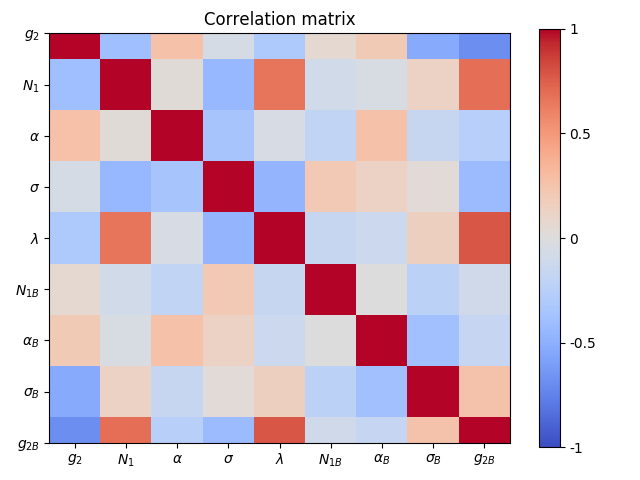
\includegraphics{pngplots/CorrelationMatrix.png}
\caption{Fitted parameter correlation matrix}
\end{figure}

\hypertarget{fit-properties}{%
\subsection{Fit properties}\label{fit-properties}}

\begin{figure}
\centering
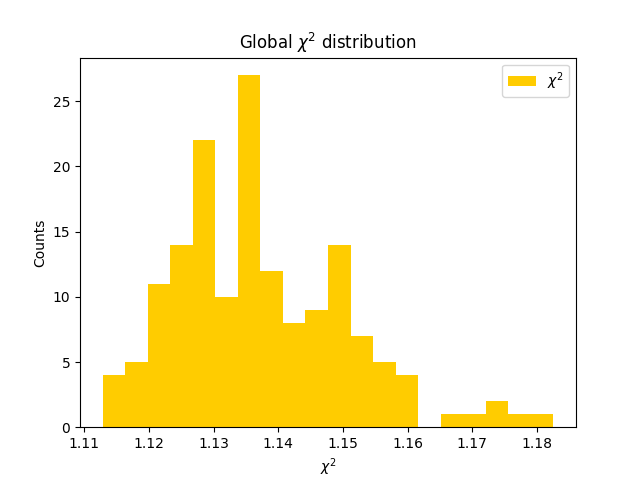
\includegraphics{pngplots/Globalchi2.png}
\caption{Global \(\chi^2\) distribution}
\end{figure}

\begin{figure}
\centering
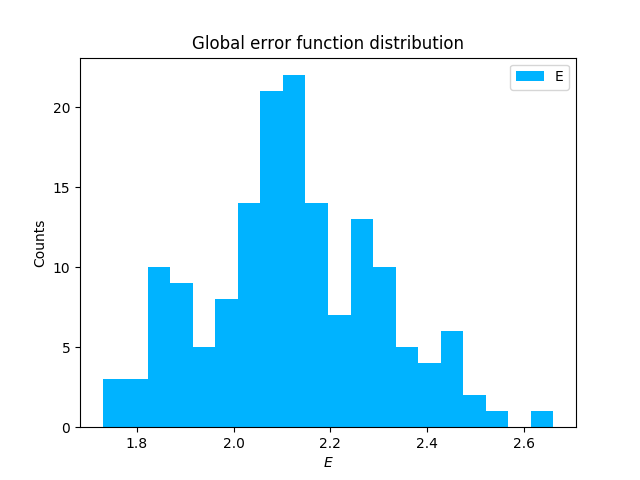
\includegraphics{pngplots/GlobalErrorFunction.png}
\caption{Global error function distribution}
\end{figure}

\begin{figure}
\centering
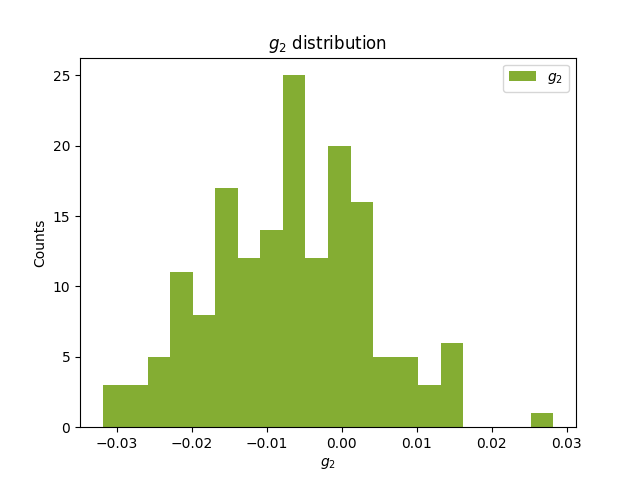
\includegraphics{pngplots/param0.png}
\caption{\(g_2\) distribution}
\end{figure}

\begin{figure}
\centering
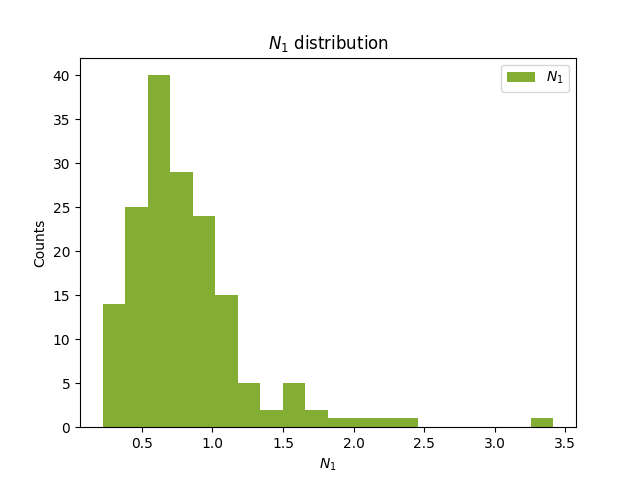
\includegraphics{pngplots/param1.png}
\caption{\(N_1\) distribution}
\end{figure}

\begin{figure}
\centering
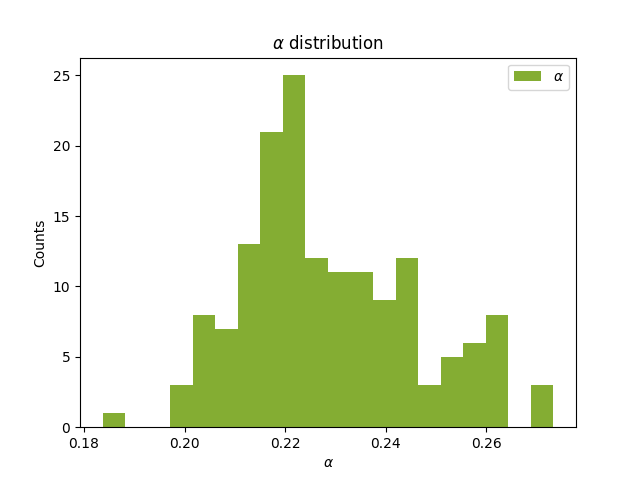
\includegraphics{pngplots/param2.png}
\caption{\(\alpha\) distribution}
\end{figure}

\begin{figure}
\centering
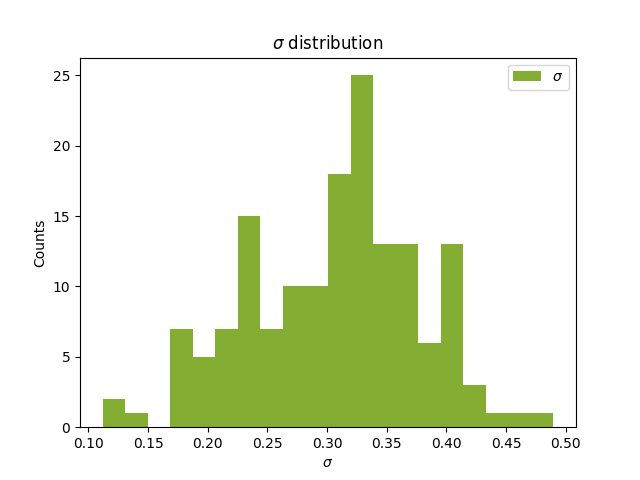
\includegraphics{pngplots/param3.png}
\caption{\(\sigma\) distribution}
\end{figure}

\begin{figure}
\centering
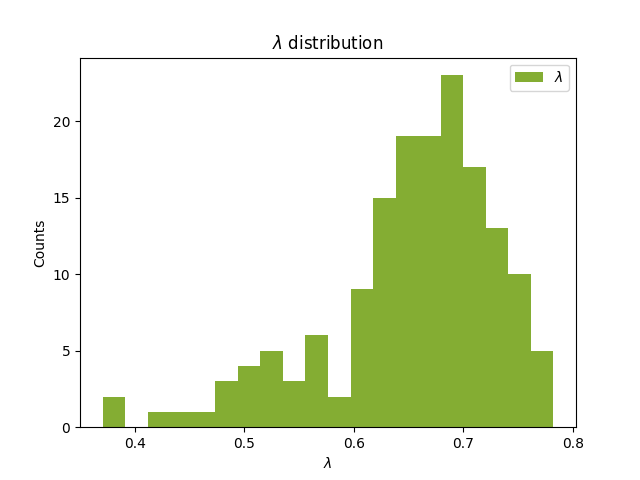
\includegraphics{pngplots/param4.png}
\caption{\(\lambda\) distribution}
\end{figure}

\begin{figure}
\centering
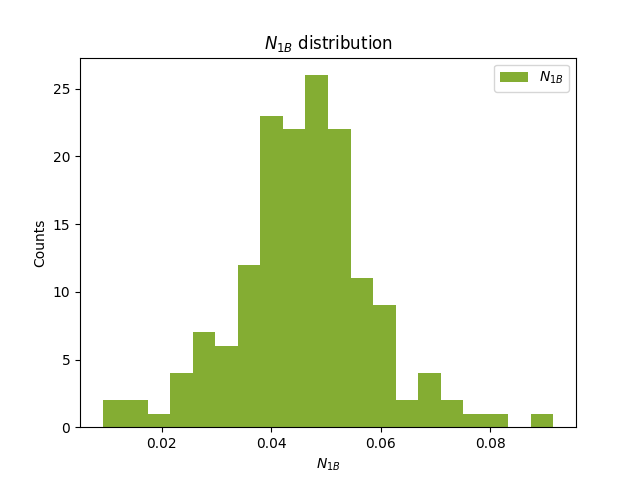
\includegraphics{pngplots/param5.png}
\caption{\(N_{1B}\) distribution}
\end{figure}

\begin{figure}
\centering
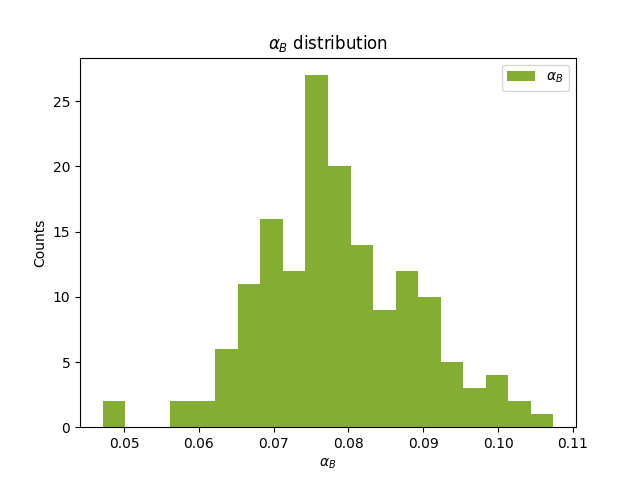
\includegraphics{pngplots/param6.png}
\caption{\(\alpha_B\) distribution}
\end{figure}

\begin{figure}
\centering
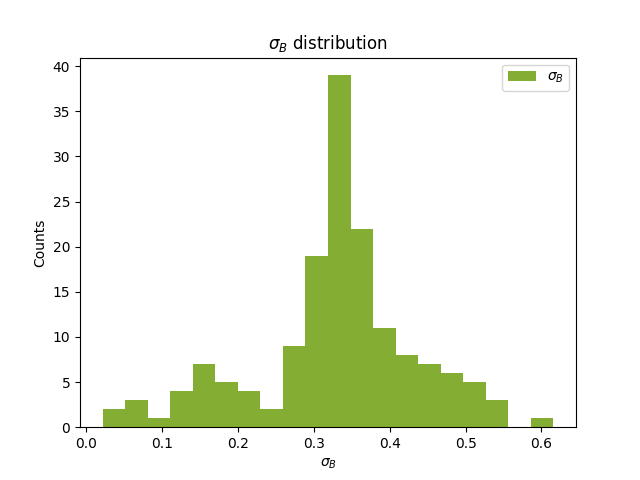
\includegraphics{pngplots/param7.png}
\caption{\(\sigma_B\) distribution}
\end{figure}

\begin{figure}
\centering
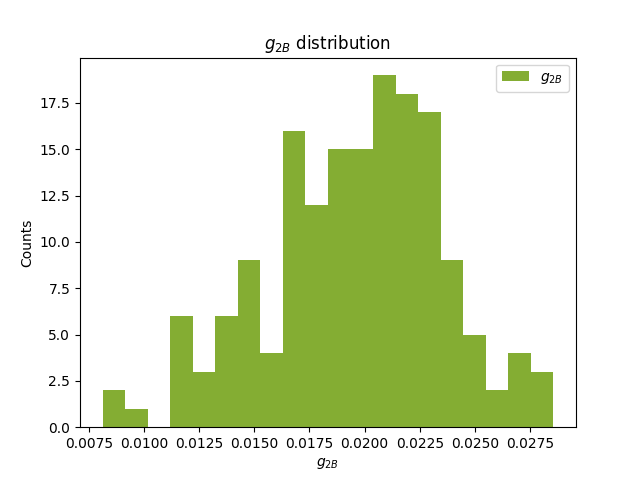
\includegraphics{pngplots/param8.png}
\caption{\(g_{2B}\) distribution}
\end{figure}

\hypertarget{table-of-chi2s}{%
\subsection{\texorpdfstring{Table of
\(\chi^2\)'s}{Table of \textbackslash chi\^{}2's}}\label{table-of-chi2s}}

\begin{table}[h]

\centering

\begin{tabular}{|c|c|c|c|c|} \hline

\textbf{Experiment} & \textbf{Number of
points} & \textbf{\(\chi_{D}^2\)} & \textbf{\(\chi_{\lambda}^2\)} & \textbf{\(\chi^2\)} \\ \hline

E605\_Q\_7\_8 & 7 & 0.5843 & 0.0 & 0.5844 \\ \hline
E605\_Q\_8\_9 & 8 & 1.442 & 0.0 & 1.442 \\ \hline
E605\_Q\_10.5\_11.5 & 10 & 0.4762 & 0.1764 & 0.6526 \\ \hline
E288\_200\_Q\_4\_5 & 4 & 0.753 & 0.8187 & 1.5717 \\ \hline
E288\_200\_Q\_5\_6 & 5 & 1.7704 & 0.2324 & 2.0028 \\ \hline
E288\_200\_Q\_6\_7 & 6 & 0.4264 & 0.1135 & 0.5399 \\ \hline
E288\_200\_Q\_7\_8 & 7 & 0.5599 & 0.0026 & 0.5626 \\ \hline
E288\_200\_Q\_8\_9 & 8 & 0.5918 & 0.0447 & 0.6365 \\ \hline
E288\_300\_Q\_4\_5 & 4 & 0.5943 & 0.4329 & 1.0271 \\ \hline
E288\_300\_Q\_5\_6 & 5 & 0.9293 & 0.1086 & 1.0379 \\ \hline
E288\_300\_Q\_6\_7 & 6 & 0.5751 & 0.0244 & 0.5995 \\ \hline
E288\_300\_Q\_7\_8 & 7 & 0.1516 & 0.0132 & 0.1648 \\ \hline
E288\_300\_Q\_8\_9 & 8 & 0.4665 & 0.0052 & 0.4717 \\ \hline
E288\_400\_Q\_5\_6 & 5 & 0.3674 & 0.0 & 0.3674 \\ \hline
E288\_400\_Q\_6\_7 & 6 & 0.1008 & 0.005 & 0.1058 \\ \hline
E288\_400\_Q\_7\_8 & 7 & 0.0245 & 0.0246 & 0.0491 \\ \hline
E288\_400\_Q\_8\_9 & 8 & 0.4599 & 0.0436 & 0.5035 \\ \hline
E288\_400\_Q\_11\_12 & 11 & 0.4904 & 0.0503 & 0.5407 \\ \hline
E288\_400\_Q\_12\_13 & 12 & 0.4861 & 0.0468 & 0.5329 \\ \hline
E288\_400\_Q\_13\_14 & 12 & 0.5925 & 0.0915 & 0.684 \\ \hline
STAR\_510 & 7 & 0.9489 & 0.0421 & 0.991 \\ \hline
CDF\_RunI & 25 & 0.5556 & 0.0727 & 0.6283 \\ \hline
CDF\_RunII & 26 & 0.9155 & 0.0022 & 0.9177 \\ \hline
D0\_RunI & 12 & 0.6224 & 0.0315 & 0.6539 \\ \hline
D0\_RunII & 5 & 0.9459 & 0.0431 & 0.9891 \\ \hline
D0\_RunIImu & 3 & 0.325 & 0.0491 & 0.3741 \\ \hline
LHCb\_7TeV & 7 & 1.1697 & 0.1975 & 1.3671 \\ \hline
LHCb\_8TeV & 7 & 0.5978 & 0.1649 & 0.7626 \\ \hline
LHCb\_13TeV & 7 & 0.8714 & 0.0422 & 0.9136 \\ \hline
CMS\_7TeV & 4 & 2.5211 & 0 & 2.5211 \\ \hline
CMS\_8TeV & 4 & 1.285 & 0.1507 & 1.4357 \\ \hline
ATLAS\_7TeV\_y\_0\_1 & 6 & 3.3163 & 0.0191 & 3.3354 \\ \hline
ATLAS\_7TeV\_y\_1\_2 & 6 & 3.5971 & 0.5985 & 4.1956 \\ \hline
ATLAS\_7TeV\_y\_2\_2.4 & 6 & 2.8794 & 0.2878 & 3.1672 \\ \hline
ATLAS\_8TeV\_y\_0\_0.4 & 6 & 2.9918 & 0.7083 & 3.7001 \\ \hline
ATLAS\_8TeV\_y\_0.4\_0.8 & 6 & 3.3963 & 0.6824 & 4.0787 \\ \hline
ATLAS\_8TeV\_y\_0.8\_1.2 & 6 & 1.5652 & 0.1759 & 1.7411 \\ \hline
ATLAS\_8TeV\_y\_1.2\_1.6 & 6 & 1.3454 & 0.2296 & 1.575 \\ \hline
ATLAS\_8TeV\_y\_1.6\_2 & 6 & 0.8918 & 0.2905 & 1.1824 \\ \hline
ATLAS\_8TeV\_y\_2\_2.4 & 6 & 0.8868 & 0.4127 & 1.2995 \\ \hline
ATLAS\_8TeV\_Q\_46\_66 & 4 & 1.8007 & 0.5584 & 2.3591 \\ \hline
ATLAS\_8TeV\_Q\_116\_150 & 8 & 0.6565 & 0.002 & 0.6585 \\ \hline
Total & 319 & - & - & 1.1092 \\ \hline

\end{tabular}

\caption{Central-replica \(\chi^2\)'s:}

\end{table}

\begin{table}[h]

\centering

\begin{tabular}{|c|c|c|c|c|} \hline

\textbf{Experiment} & \textbf{Number of
points} & \textbf{\(\chi_{D}^2\)} & \textbf{\(\chi_{\lambda}^2\)} & \textbf{\(\chi^2\)} \\ \hline

E605\_Q\_7\_8 & 7 & 0.7629 & 0.0777 & 0.8406 \\ \hline
E605\_Q\_8\_9 & 8 & 1.5305 & 0.0093 & 1.5398 \\ \hline
E605\_Q\_10.5\_11.5 & 10 & 0.3546 & 0.1622 & 0.5169 \\ \hline
E288\_200\_Q\_4\_5 & 4 & 0.4285 & 0.247 & 0.6755 \\ \hline
E288\_200\_Q\_5\_6 & 5 & 1.2808 & 0.1147 & 1.3955 \\ \hline
E288\_200\_Q\_6\_7 & 6 & 0.3381 & 0.0694 & 0.4075 \\ \hline
E288\_200\_Q\_7\_8 & 7 & 0.57 & 0.0076 & 0.5776 \\ \hline
E288\_200\_Q\_8\_9 & 8 & 0.8081 & 0.017 & 0.8252 \\ \hline
E288\_300\_Q\_4\_5 & 4 & 0.4409 & 0.0879 & 0.5289 \\ \hline
E288\_300\_Q\_5\_6 & 5 & 0.7565 & 0.055 & 0.8114 \\ \hline
E288\_300\_Q\_6\_7 & 6 & 0.5159 & 0.0234 & 0.5393 \\ \hline
E288\_300\_Q\_7\_8 & 7 & 0.1467 & 0.0145 & 0.1611 \\ \hline
E288\_300\_Q\_8\_9 & 8 & 0.392 & 0.01 & 0.402 \\ \hline
E288\_400\_Q\_5\_6 & 5 & 0.5063 & 0.0144 & 0.5207 \\ \hline
E288\_400\_Q\_6\_7 & 6 & 0.1144 & 0.0094 & 0.1238 \\ \hline
E288\_400\_Q\_7\_8 & 7 & 0.0359 & 0.0185 & 0.0545 \\ \hline
E288\_400\_Q\_8\_9 & 8 & 0.6179 & 0.0297 & 0.6477 \\ \hline
E288\_400\_Q\_11\_12 & 11 & 0.7325 & 0.0677 & 0.8002 \\ \hline
E288\_400\_Q\_12\_13 & 12 & 0.776 & 0.0509 & 0.8269 \\ \hline
E288\_400\_Q\_13\_14 & 12 & 1.1021 & 0.0589 & 1.161 \\ \hline
STAR\_510 & 7 & 0.9636 & 0.075 & 1.0386 \\ \hline
CDF\_RunI & 25 & 0.5218 & 0.0746 & 0.5964 \\ \hline
CDF\_RunII & 26 & 0.9909 & 0.0 & 0.9909 \\ \hline
D0\_RunI & 12 & 0.6515 & 0.0279 & 0.6794 \\ \hline
D0\_RunII & 5 & 1.3618 & 0.0485 & 1.4103 \\ \hline
D0\_RunIImu & 3 & 0.1155 & 0.018 & 0.1335 \\ \hline
LHCb\_7TeV & 7 & 1.0434 & 0.2184 & 1.2618 \\ \hline
LHCb\_8TeV & 7 & 0.5283 & 0.1704 & 0.6987 \\ \hline
LHCb\_13TeV & 7 & 0.947 & 0.041 & 0.988 \\ \hline
CMS\_7TeV & 4 & 2.5098 & 0 & 2.5098 \\ \hline
CMS\_8TeV & 4 & 1.2751 & 0.1493 & 1.4244 \\ \hline
ATLAS\_7TeV\_y\_0\_1 & 6 & 3.228 & 0.0201 & 3.2481 \\ \hline
ATLAS\_7TeV\_y\_1\_2 & 6 & 3.5075 & 0.6001 & 4.1076 \\ \hline
ATLAS\_7TeV\_y\_2\_2.4 & 6 & 2.9771 & 0.2997 & 3.2768 \\ \hline
ATLAS\_8TeV\_y\_0\_0.4 & 6 & 2.9443 & 0.7127 & 3.6569 \\ \hline
ATLAS\_8TeV\_y\_0.4\_0.8 & 6 & 3.315 & 0.6891 & 4.0041 \\ \hline
ATLAS\_8TeV\_y\_0.8\_1.2 & 6 & 1.5297 & 0.1784 & 1.7081 \\ \hline
ATLAS\_8TeV\_y\_1.2\_1.6 & 6 & 1.3111 & 0.2324 & 1.5435 \\ \hline
ATLAS\_8TeV\_y\_1.6\_2 & 6 & 0.8455 & 0.2862 & 1.1317 \\ \hline
ATLAS\_8TeV\_y\_2\_2.4 & 6 & 0.7733 & 0.3493 & 1.1226 \\ \hline
ATLAS\_8TeV\_Q\_46\_66 & 4 & 1.8165 & 0.5561 & 2.3725 \\ \hline
ATLAS\_8TeV\_Q\_116\_150 & 8 & 0.6605 & 0.0014 & 0.662 \\ \hline
Total & 319 & - & - & 1.1253 \\ \hline

\end{tabular}

\caption{Mean-replica \(\chi^2\)'s:}

\end{table}

\begin{table}[h]

\centering

\begin{tabular}{|c|c|c|c|c|} \hline

\textbf{Experiment} & \textbf{Number of
points} & \textbf{\(\chi_{D}^2\)} & \textbf{\(\chi_{\lambda}^2\)} & \textbf{\(\chi^2\)} \\ \hline

E605\_Q\_7\_8 & 7 & 0.5039 \(\pm\) 0.2099 & 0.1252 \(\pm\)
0.1631 & 0.629 \(\pm\) 0.125 \\ \hline
E605\_Q\_8\_9 & 8 & 1.3308 \(\pm\) 0.2698 & 0.0851 \(\pm\)
0.1245 & 1.4159 \(\pm\) 0.247 \\ \hline
E605\_Q\_10.5\_11.5 & 10 & 0.4695 \(\pm\) 0.3635 & 0.2562 \(\pm\)
0.305 & 0.7257 \(\pm\) 0.1688 \\ \hline
E288\_200\_Q\_4\_5 & 4 & 0.3794 \(\pm\) 1.374 & 1.1706 \(\pm\)
1.302 & 1.55 \(\pm\) 0.3598 \\ \hline
E288\_200\_Q\_5\_6 & 5 & 1.5756 \(\pm\) 0.7851 & 0.4829 \(\pm\)
0.7066 & 2.0585 \(\pm\) 0.2393 \\ \hline
E288\_200\_Q\_6\_7 & 6 & 0.2222 \(\pm\) 0.4187 & 0.3515 \(\pm\)
0.4016 & 0.5738 \(\pm\) 0.1223 \\ \hline
E288\_200\_Q\_7\_8 & 7 & 0.4423 \(\pm\) 0.2465 & 0.151 \(\pm\)
0.1922 & 0.5933 \(\pm\) 0.1644 \\ \hline
E288\_200\_Q\_8\_9 & 8 & 0.5161 \(\pm\) 0.1544 & 0.1325 \(\pm\)
0.1431 & 0.6487 \(\pm\) 0.0767 \\ \hline
E288\_300\_Q\_4\_5 & 4 & 0.3173 \(\pm\) 0.9901 & 0.6951 \(\pm\)
0.9038 & 1.0124 \(\pm\) 0.2539 \\ \hline
E288\_300\_Q\_5\_6 & 5 & 0.7531 \(\pm\) 0.5016 & 0.3447 \(\pm\)
0.455 & 1.0977 \(\pm\) 0.1619 \\ \hline
E288\_300\_Q\_6\_7 & 6 & 0.4348 \(\pm\) 0.3404 & 0.2076 \(\pm\)
0.3019 & 0.6424 \(\pm\) 0.1511 \\ \hline
E288\_300\_Q\_7\_8 & 7 & 0.0164 \(\pm\) 0.2385 & 0.1708 \(\pm\)
0.2217 & 0.1873 \(\pm\) 0.0659 \\ \hline
E288\_300\_Q\_8\_9 & 8 & 0.3882 \(\pm\) 0.1501 & 0.1012 \(\pm\)
0.1441 & 0.4895 \(\pm\) 0.0782 \\ \hline
E288\_400\_Q\_5\_6 & 5 & 0.2382 \(\pm\) 0.3189 & 0.2074 \(\pm\)
0.2776 & 0.4456 \(\pm\) 0.1397 \\ \hline
E288\_400\_Q\_6\_7 & 6 & 0.0076 \(\pm\) 0.1926 & 0.1459 \(\pm\)
0.2114 & 0.1534 \(\pm\) 0.1036 \\ \hline
E288\_400\_Q\_7\_8 & 7 & -0.0415 \(\pm\) 0.1829 & 0.1322 \(\pm\)
0.1637 & 0.0907 \(\pm\) 0.0909 \\ \hline
E288\_400\_Q\_8\_9 & 8 & 0.4131 \(\pm\) 0.2158 & 0.1361 \(\pm\)
0.1915 & 0.5492 \(\pm\) 0.1332 \\ \hline
E288\_400\_Q\_11\_12 & 11 & 0.4925 \(\pm\) 0.2081 & 0.1079 \(\pm\)
0.1213 & 0.6004 \(\pm\) 0.1792 \\ \hline
E288\_400\_Q\_12\_13 & 12 & 0.4516 \(\pm\) 0.1399 & 0.1154 \(\pm\)
0.1335 & 0.567 \(\pm\) 0.0507 \\ \hline
E288\_400\_Q\_13\_14 & 12 & 0.571 \(\pm\) 0.1358 & 0.1229 \(\pm\)
0.1226 & 0.6939 \(\pm\) 0.0611 \\ \hline
STAR\_510 & 7 & 0.8668 \(\pm\) 0.2057 & 0.1558 \(\pm\) 0.2081 & 1.0227
\(\pm\) 0.0642 \\ \hline
CDF\_RunI & 25 & 0.5246 \(\pm\) 0.1125 & 0.1091 \(\pm\) 0.1088 & 0.6336
\(\pm\) 0.022 \\ \hline
CDF\_RunII & 26 & 0.8943 \(\pm\) 0.1091 & 0.0462 \(\pm\) 0.0563 & 0.9405
\(\pm\) 0.0891 \\ \hline
D0\_RunI & 12 & 0.5689 \(\pm\) 0.1281 & 0.0913 \(\pm\) 0.1235 & 0.6601
\(\pm\) 0.0312 \\ \hline
D0\_RunII & 5 & 0.7756 \(\pm\) 0.3753 & 0.2212 \(\pm\) 0.2936 & 0.9968
\(\pm\) 0.2163 \\ \hline
D0\_RunIImu & 3 & -0.1678 \(\pm\) 0.5949 & 0.5601 \(\pm\)
0.5417 & 0.3923 \(\pm\) 0.2268 \\ \hline
LHCb\_7TeV & 7 & 0.9692 \(\pm\) 0.3323 & 0.3989 \(\pm\) 0.3307 & 1.3681
\(\pm\) 0.0334 \\ \hline
LHCb\_8TeV & 7 & 0.487 \(\pm\) 0.4113 & 0.3126 \(\pm\) 0.386 & 0.7997
\(\pm\) 0.1448 \\ \hline
LHCb\_13TeV & 7 & 0.8217 \(\pm\) 0.2287 & 0.137 \(\pm\) 0.2171 & 0.9587
\(\pm\) 0.0884 \\ \hline
CMS\_7TeV & 4 & 2.5221 \(\pm\) 0.016 & 0.0 \(\pm\) 0.0 & 2.5221 \(\pm\)
0.016 \\ \hline
CMS\_8TeV & 4 & 1.2044 \(\pm\) 0.2317 & 0.225 \(\pm\) 0.2213 & 1.4294
\(\pm\) 0.0663 \\ \hline
ATLAS\_7TeV\_y\_0\_1 & 6 & 3.2744 \(\pm\) 0.3456 & 0.0961 \(\pm\)
0.1181 & 3.3706 \(\pm\) 0.3166 \\ \hline
ATLAS\_7TeV\_y\_1\_2 & 6 & 3.6787 \(\pm\) 0.3522 & 0.5943 \(\pm\)
0.3124 & 4.2729 \(\pm\) 0.1542 \\ \hline
ATLAS\_7TeV\_y\_2\_2.4 & 6 & 2.8927 \(\pm\) 0.1796 & 0.3245 \(\pm\)
0.1484 & 3.2172 \(\pm\) 0.1019 \\ \hline
ATLAS\_8TeV\_y\_0\_0.4 & 6 & 2.9351 \(\pm\) 0.4828 & 0.777 \(\pm\)
0.4141 & 3.7122 \(\pm\) 0.1977 \\ \hline
ATLAS\_8TeV\_y\_0.4\_0.8 & 6 & 3.3104 \(\pm\) 0.517 & 0.8081 \(\pm\)
0.5027 & 4.1185 \(\pm\) 0.104 \\ \hline
ATLAS\_8TeV\_y\_0.8\_1.2 & 6 & 1.5549 \(\pm\) 0.2321 & 0.2175 \(\pm\)
0.2092 & 1.7724 \(\pm\) 0.0724 \\ \hline
ATLAS\_8TeV\_y\_1.2\_1.6 & 6 & 1.3247 \(\pm\) 0.2555 & 0.2822 \(\pm\)
0.2359 & 1.6068 \(\pm\) 0.1018 \\ \hline
ATLAS\_8TeV\_y\_1.6\_2 & 6 & 0.9726 \(\pm\) 0.411 & 0.309 \(\pm\)
0.288 & 1.2816 \(\pm\) 0.2679 \\ \hline
ATLAS\_8TeV\_y\_2\_2.4 & 6 & 0.9173 \(\pm\) 0.4795 & 0.5105 \(\pm\)
0.3264 & 1.4278 \(\pm\) 0.3287 \\ \hline
ATLAS\_8TeV\_Q\_46\_66 & 4 & 1.6317 \(\pm\) 0.6415 & 0.7217 \(\pm\)
0.6262 & 2.3534 \(\pm\) 0.1049 \\ \hline
ATLAS\_8TeV\_Q\_116\_150 & 8 & 0.559 \(\pm\) 0.1801 & 0.107 \(\pm\)
0.1795 & 0.6659 \(\pm\) 0.0184 \\ \hline
Total & 319 & - & - & 1.1393 \(\pm\) 0.018 \\ \hline

\end{tabular}

\caption{Average-over-replicas \(\chi^2\)'s:}

\end{table}

\hypertarget{tmds-in-k_t-space}{%
\subsection{\texorpdfstring{TMDs in \(k_T\)
space}{TMDs in k\_T space}}\label{tmds-in-k_t-space}}

\begin{figure}
\centering
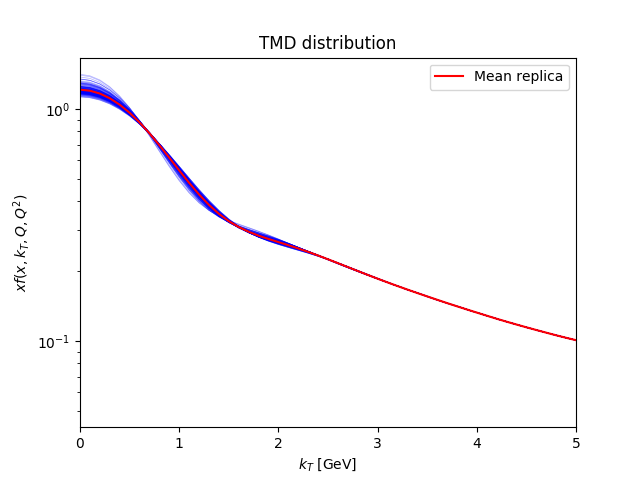
\includegraphics{pngplots/tmd_1_2_0.001.png}
\caption{TMD PDF of the \(d\) at \(Q = 2\) GeV and \(x = 0.001\)}
\end{figure}

\begin{figure}
\centering
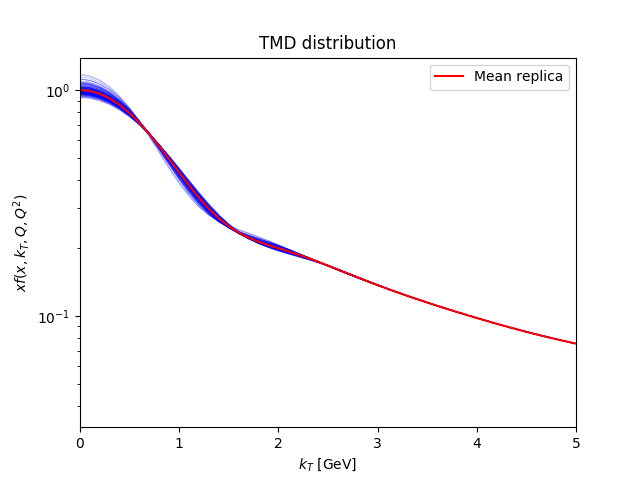
\includegraphics{pngplots/tmd_1_2_0.01.png}
\caption{TMD PDF of the \(d\) at \(Q = 2\) GeV and \(x = 0.01\)}
\end{figure}

\begin{figure}
\centering
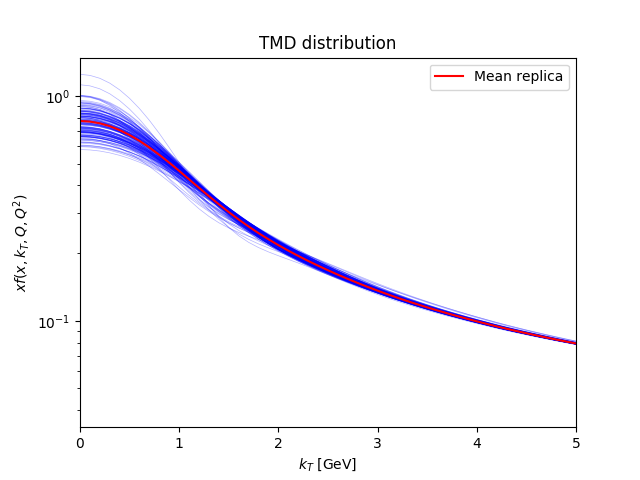
\includegraphics{pngplots/tmd_1_2_0.1.png}
\caption{TMD PDF of the \(d\) at \(Q = 2\) GeV and \(x = 0.1\)}
\end{figure}

\begin{figure}
\centering
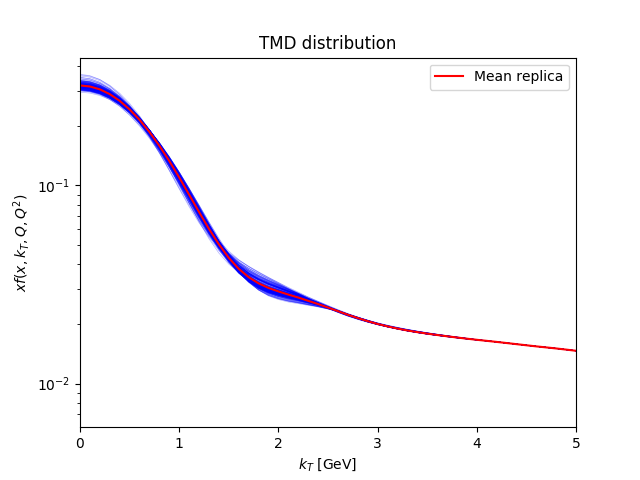
\includegraphics{pngplots/tmd_1_2_0.5.png}
\caption{TMD PDF of the \(d\) at \(Q = 2\) GeV and \(x = 0.5\)}
\end{figure}

\begin{figure}
\centering
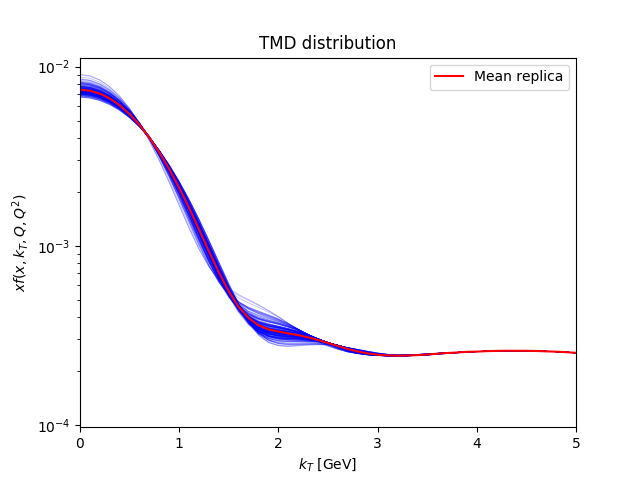
\includegraphics{pngplots/tmd_1_2_0.9.png}
\caption{TMD PDF of the \(d\) at \(Q = 2\) GeV and \(x = 0.9\)}
\end{figure}

\hypertarget{data-theory-comparison}{%
\subsection{Data-theory comparison}\label{data-theory-comparison}}

\begin{figure}
\centering
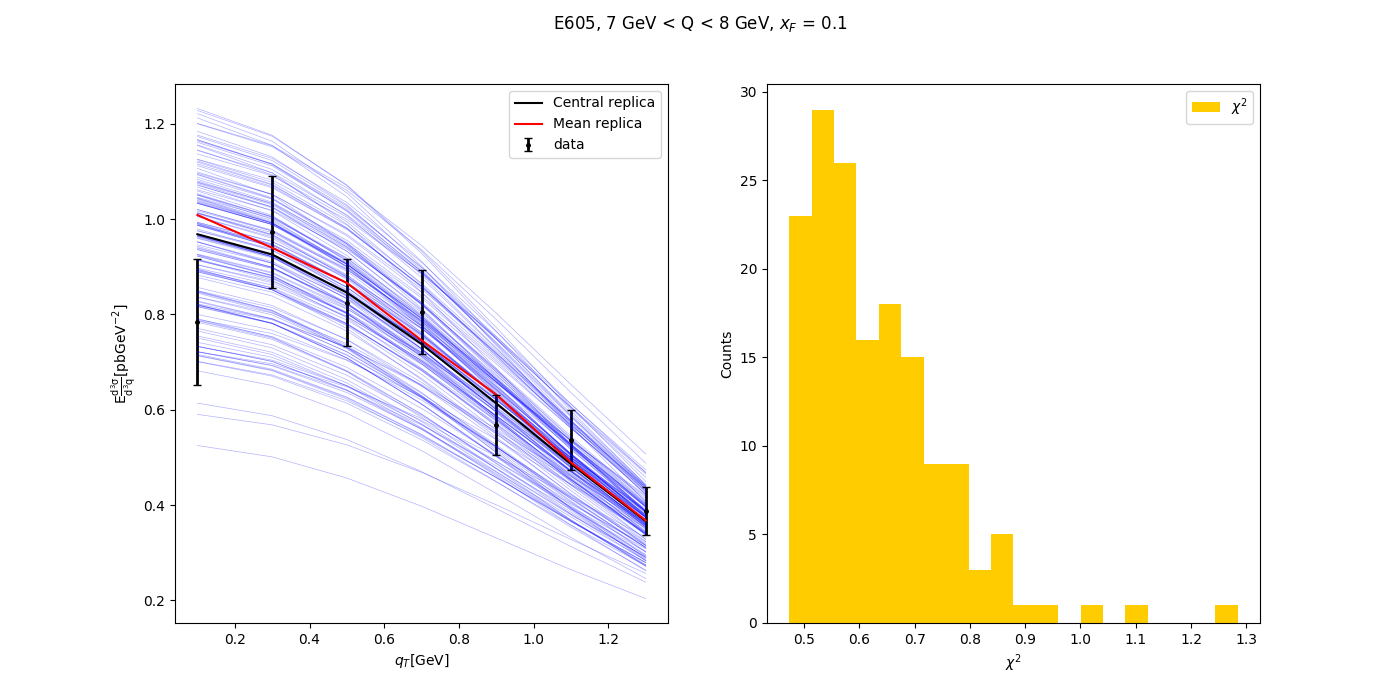
\includegraphics{pngplots/E605_Q_7_8.png}
\caption{E605\_Q\_7\_8 data-theory comparison}
\end{figure}

\begin{figure}
\centering
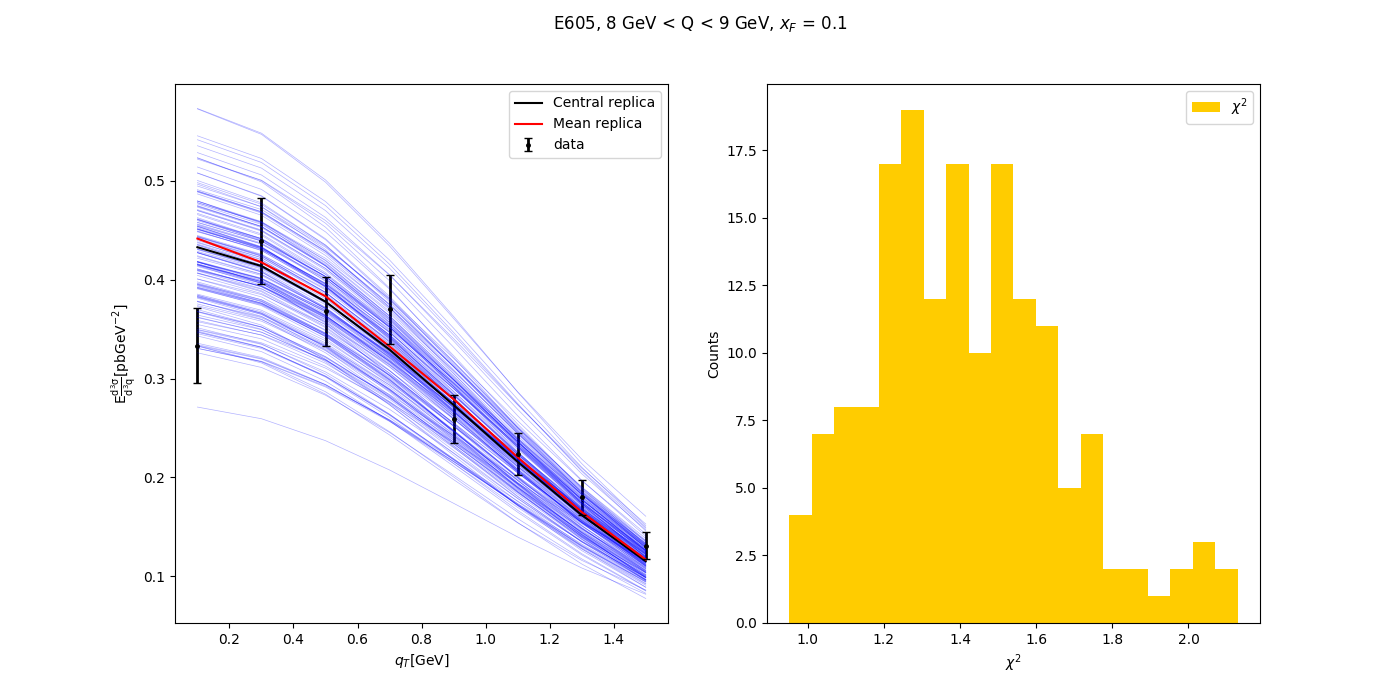
\includegraphics{pngplots/E605_Q_8_9.png}
\caption{E605\_Q\_8\_9 data-theory comparison}
\end{figure}

\begin{figure}
\centering
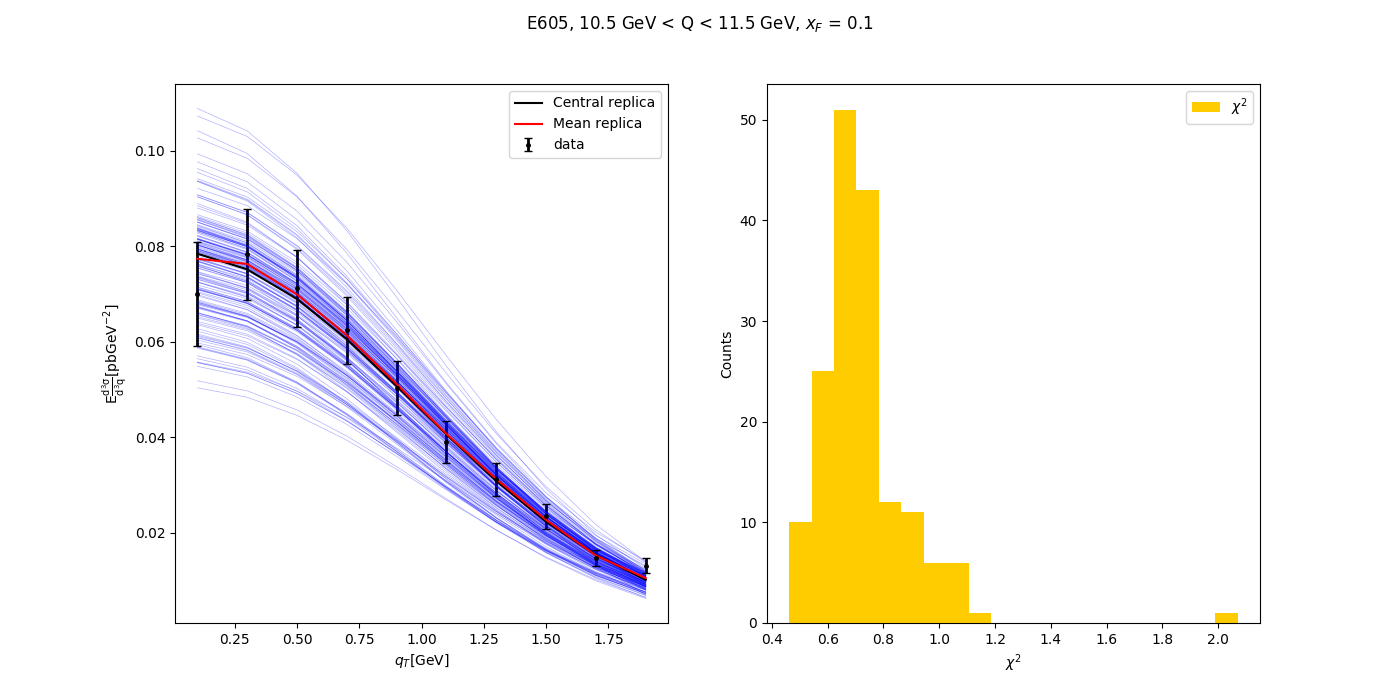
\includegraphics{pngplots/E605_Q_10.5_11.5.png}
\caption{E605\_Q\_10.5\_11.5 data-theory comparison}
\end{figure}

\begin{figure}
\centering
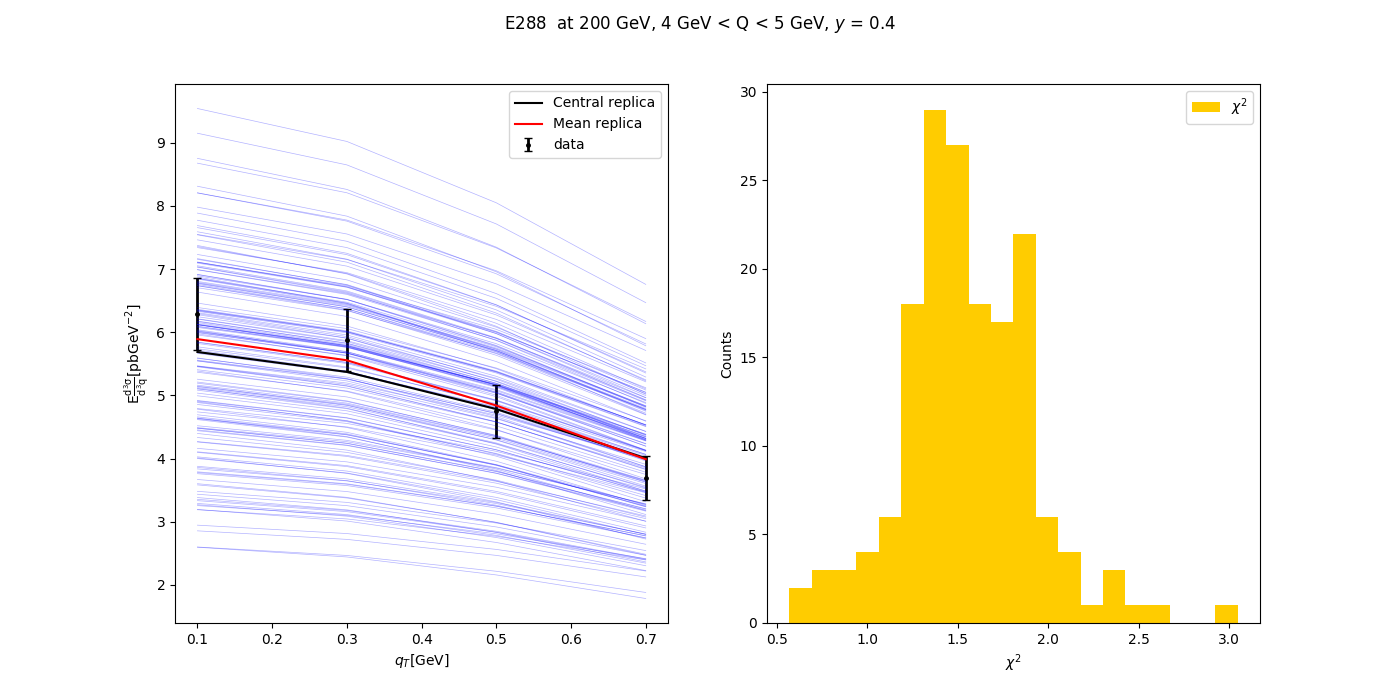
\includegraphics{pngplots/E288_200_Q_4_5.png}
\caption{E288\_200\_Q\_4\_5 data-theory comparison}
\end{figure}

\begin{figure}
\centering
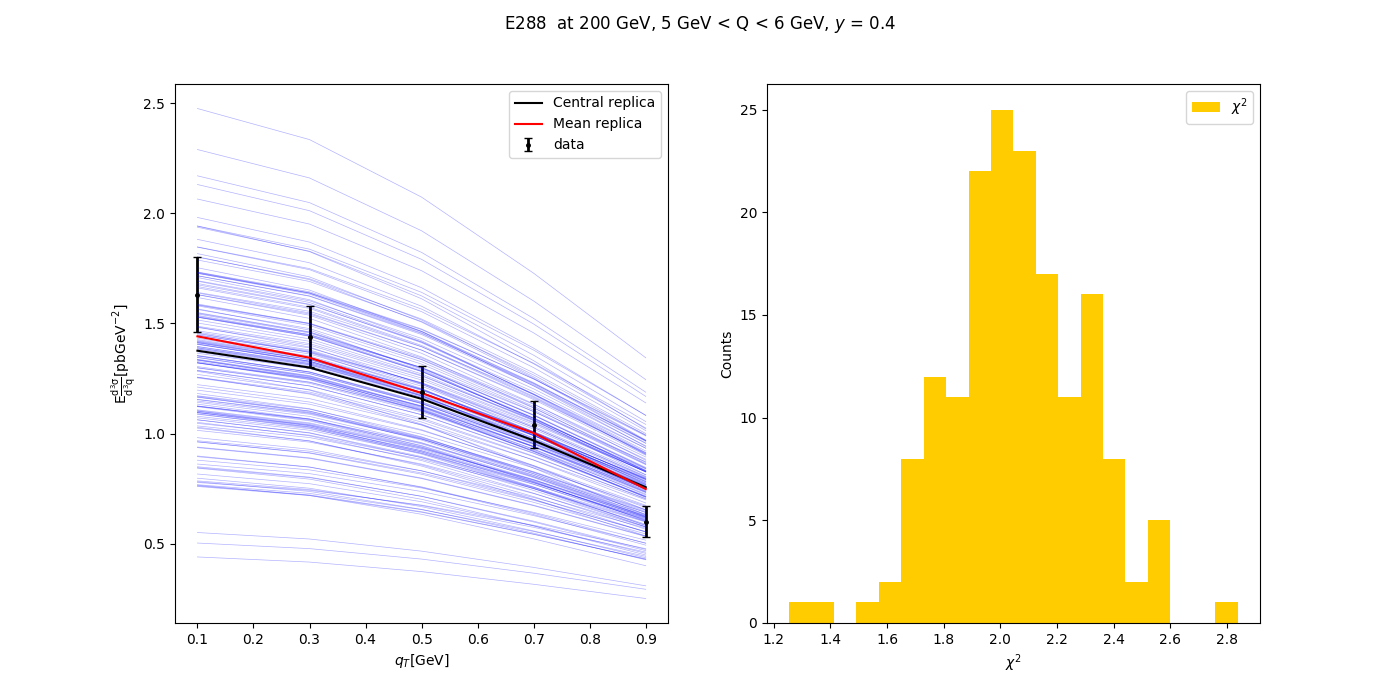
\includegraphics{pngplots/E288_200_Q_5_6.png}
\caption{E288\_200\_Q\_5\_6 data-theory comparison}
\end{figure}

\begin{figure}
\centering
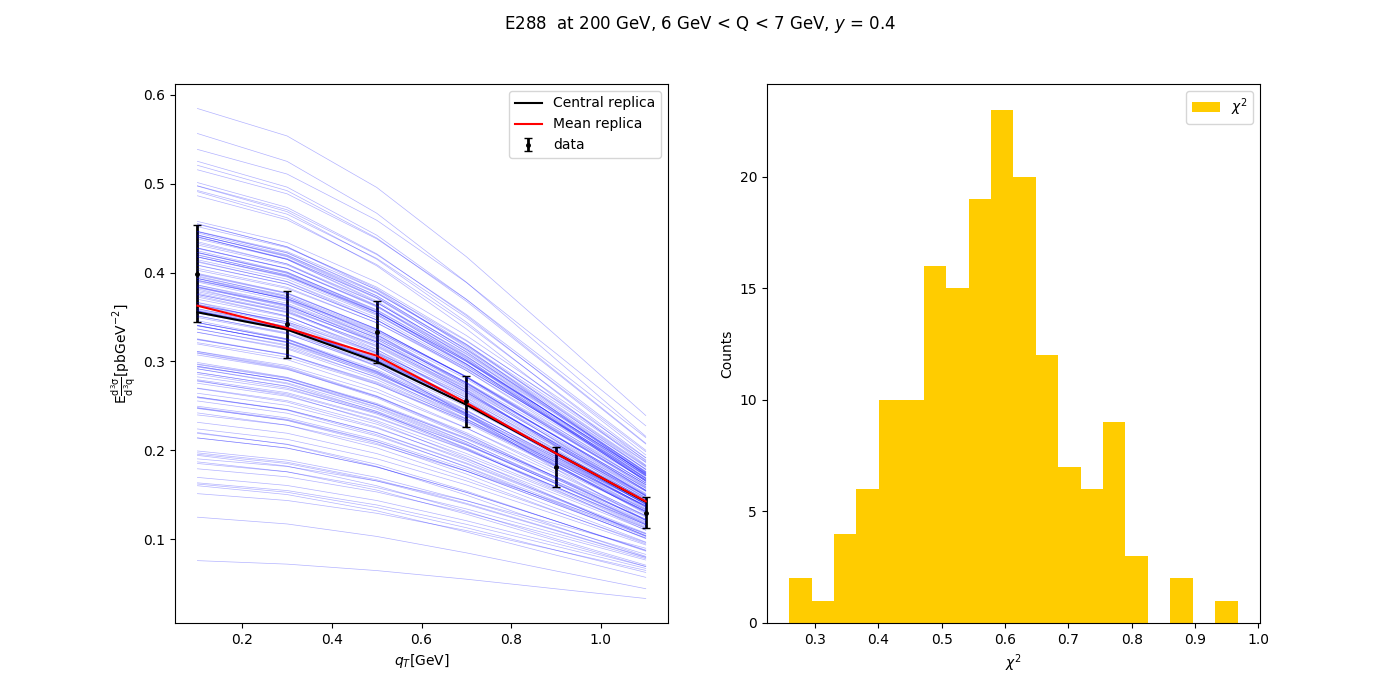
\includegraphics{pngplots/E288_200_Q_6_7.png}
\caption{E288\_200\_Q\_6\_7 data-theory comparison}
\end{figure}

\begin{figure}
\centering
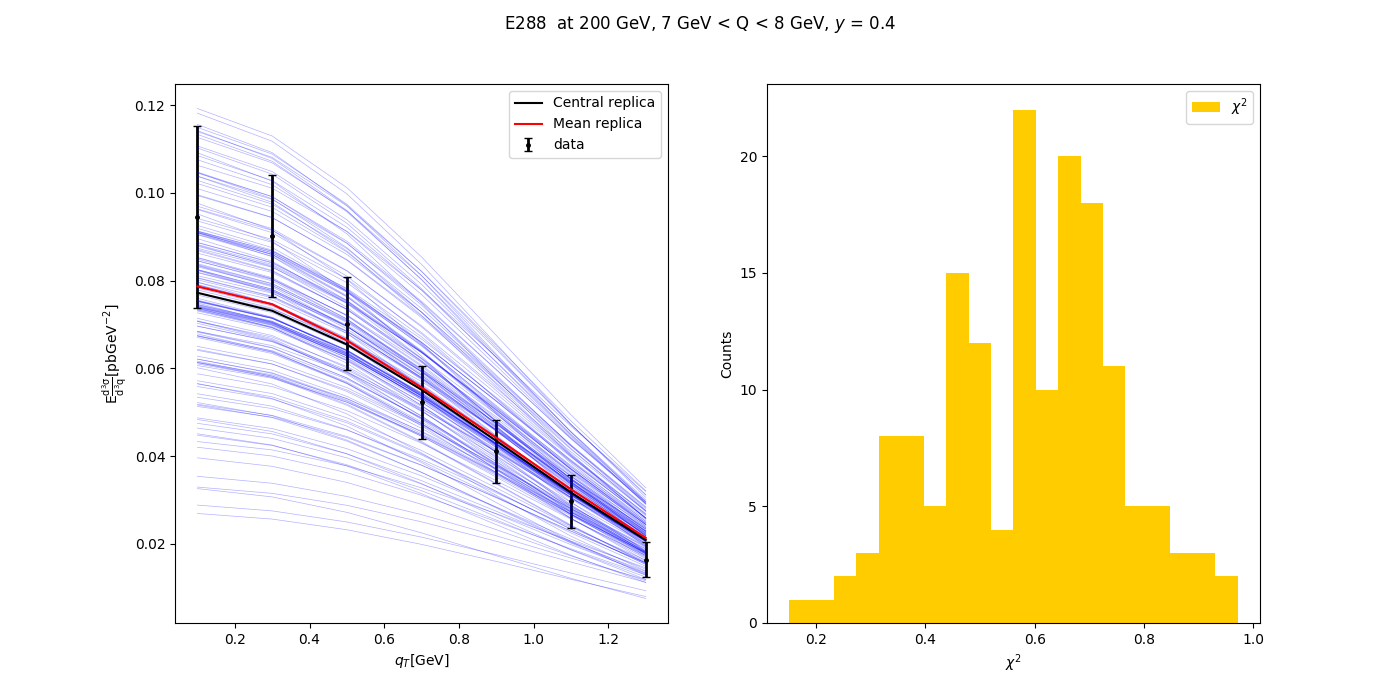
\includegraphics{pngplots/E288_200_Q_7_8.png}
\caption{E288\_200\_Q\_7\_8 data-theory comparison}
\end{figure}

\begin{figure}
\centering
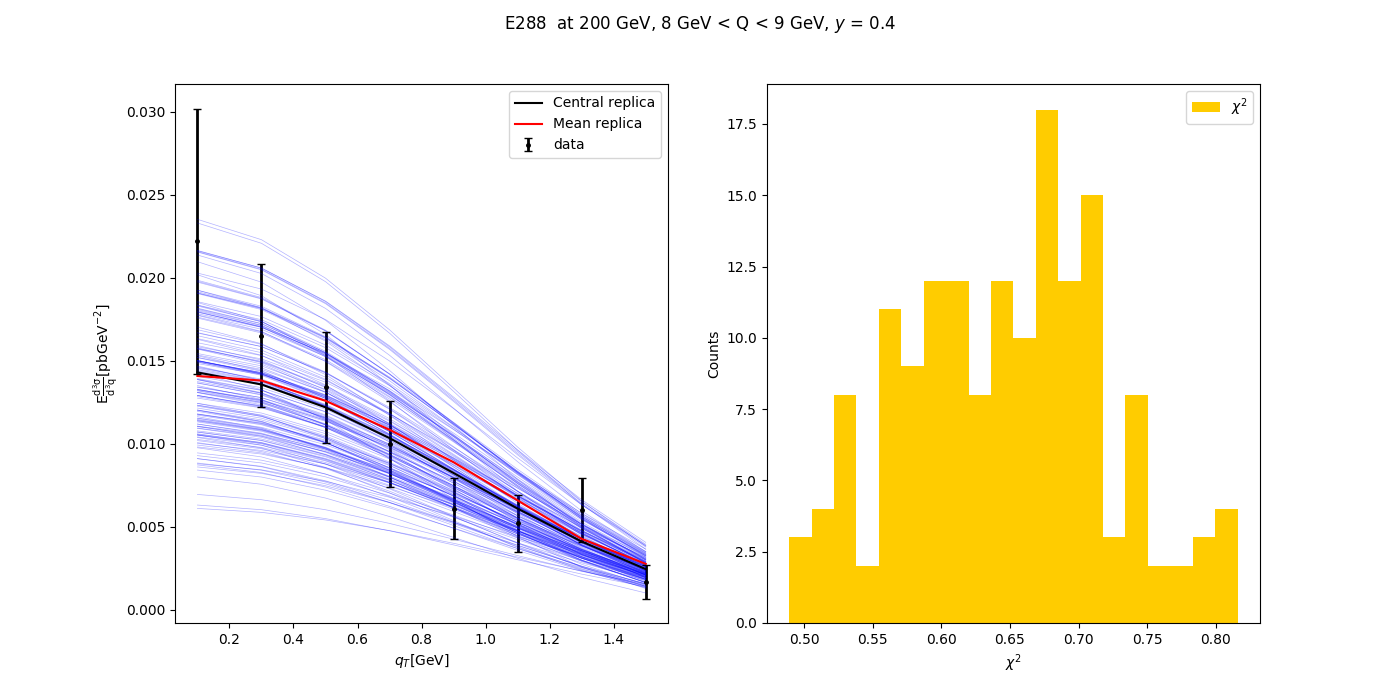
\includegraphics{pngplots/E288_200_Q_8_9.png}
\caption{E288\_200\_Q\_8\_9 data-theory comparison}
\end{figure}

\begin{figure}
\centering
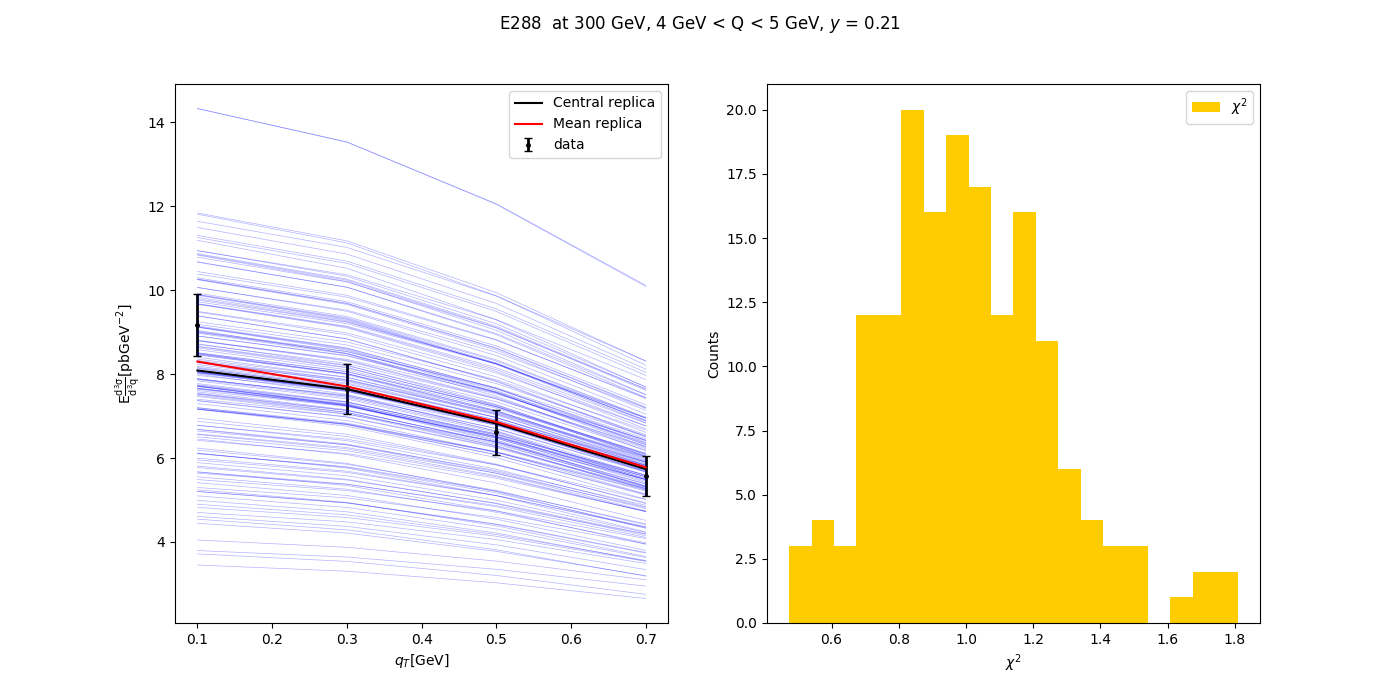
\includegraphics{pngplots/E288_300_Q_4_5.png}
\caption{E288\_300\_Q\_4\_5 data-theory comparison}
\end{figure}

\begin{figure}
\centering
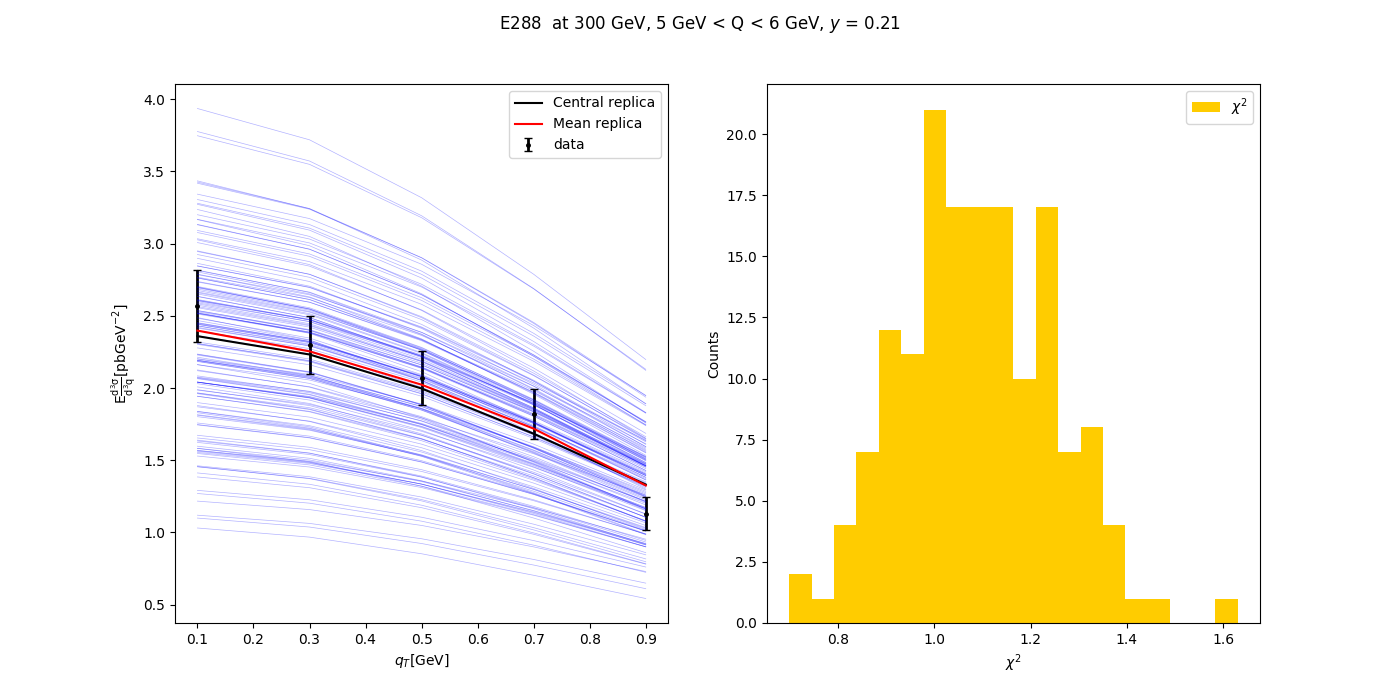
\includegraphics{pngplots/E288_300_Q_5_6.png}
\caption{E288\_300\_Q\_5\_6 data-theory comparison}
\end{figure}

\begin{figure}
\centering
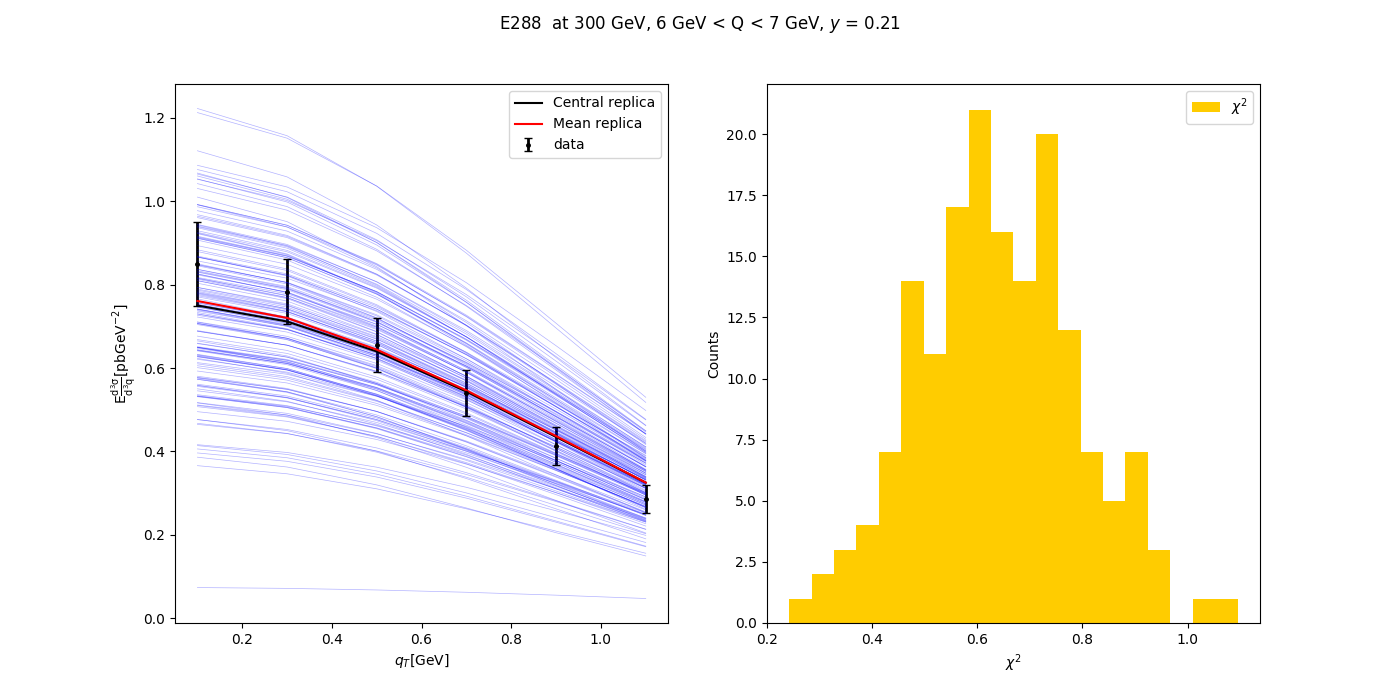
\includegraphics{pngplots/E288_300_Q_6_7.png}
\caption{E288\_300\_Q\_6\_7 data-theory comparison}
\end{figure}

\begin{figure}
\centering
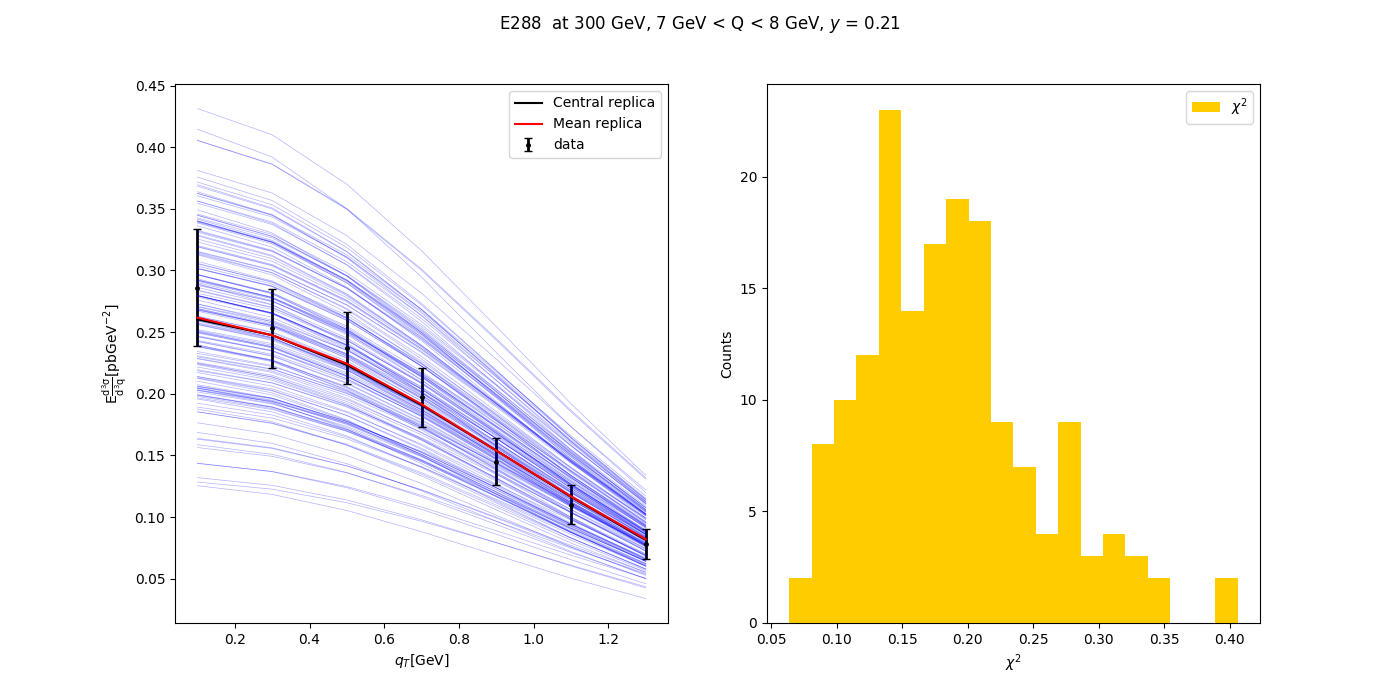
\includegraphics{pngplots/E288_300_Q_7_8.png}
\caption{E288\_300\_Q\_7\_8 data-theory comparison}
\end{figure}

\begin{figure}
\centering
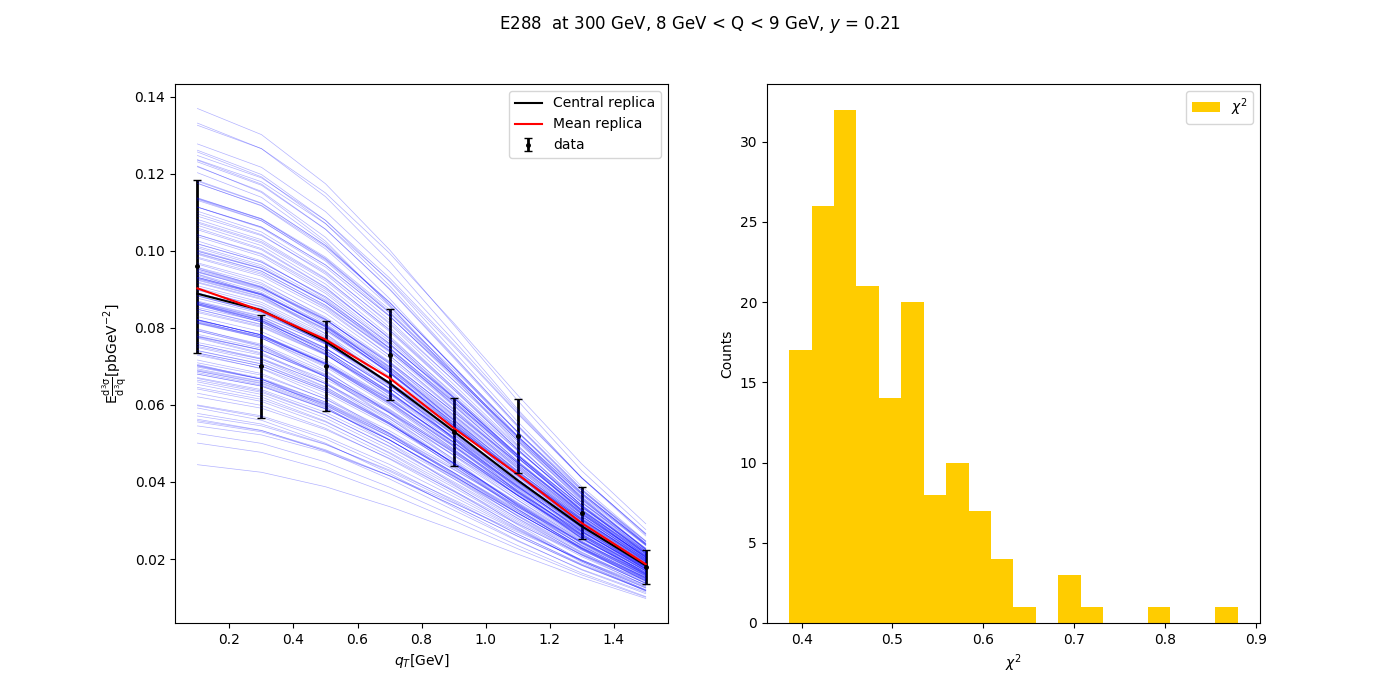
\includegraphics{pngplots/E288_300_Q_8_9.png}
\caption{E288\_300\_Q\_8\_9 data-theory comparison}
\end{figure}

\begin{figure}
\centering
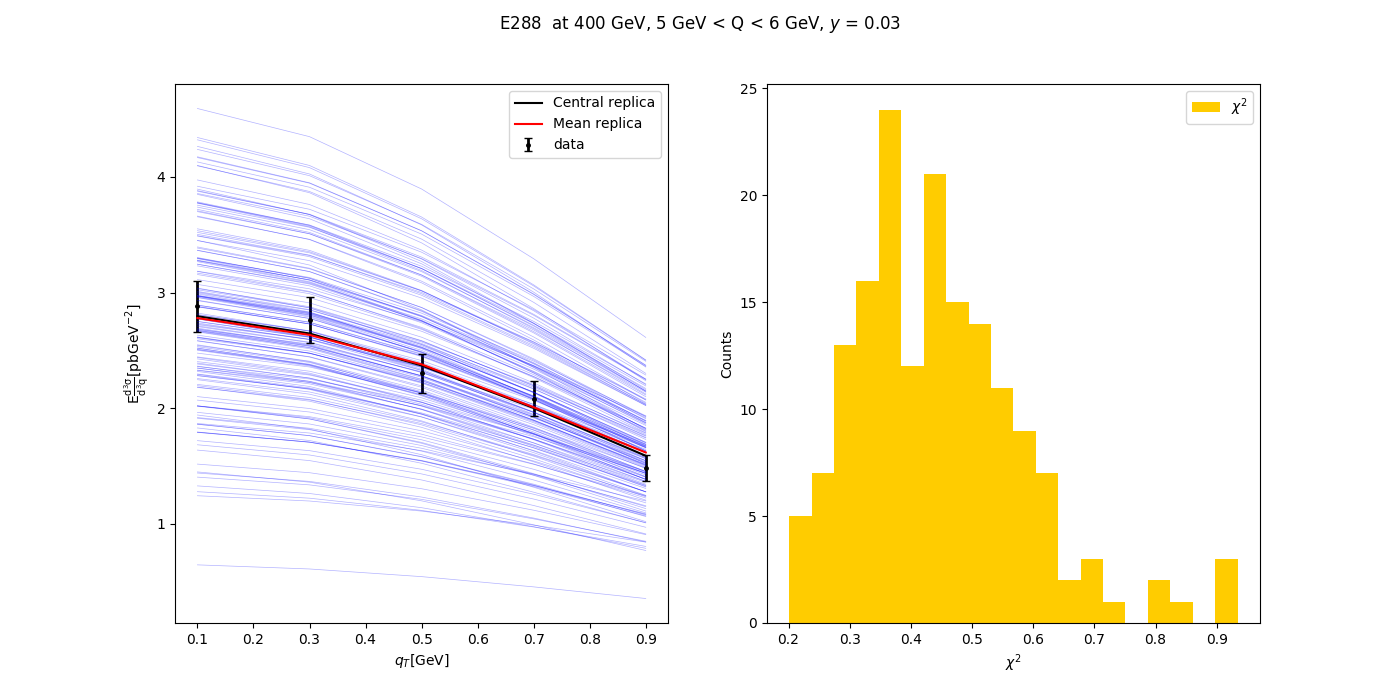
\includegraphics{pngplots/E288_400_Q_5_6.png}
\caption{E288\_400\_Q\_5\_6 data-theory comparison}
\end{figure}

\begin{figure}
\centering
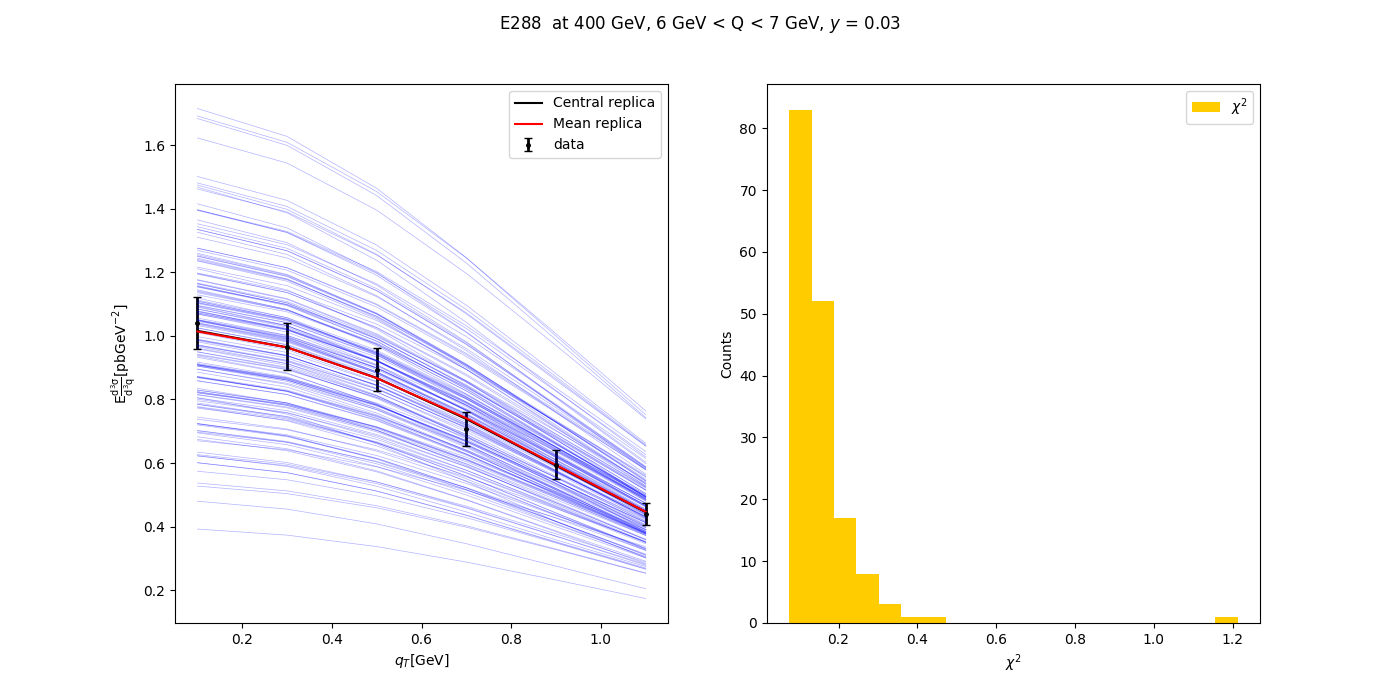
\includegraphics{pngplots/E288_400_Q_6_7.png}
\caption{E288\_400\_Q\_6\_7 data-theory comparison}
\end{figure}

\begin{figure}
\centering
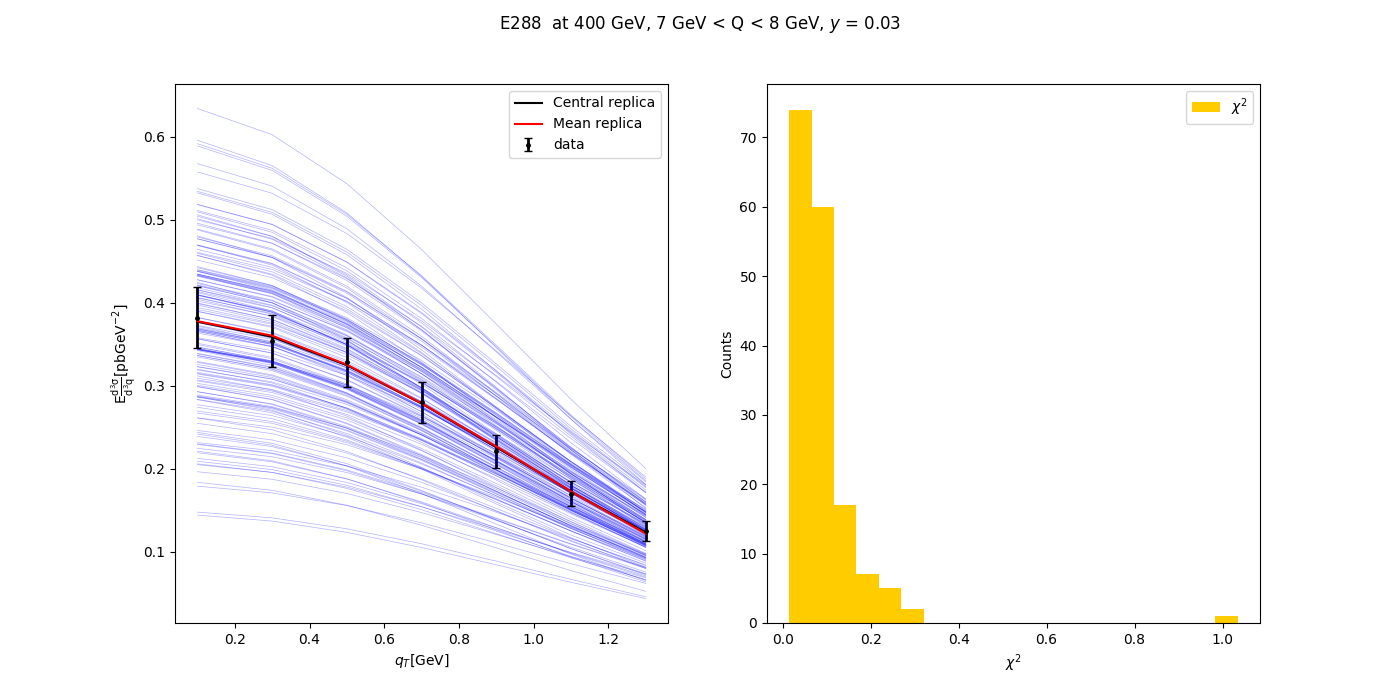
\includegraphics{pngplots/E288_400_Q_7_8.png}
\caption{E288\_400\_Q\_7\_8 data-theory comparison}
\end{figure}

\begin{figure}
\centering
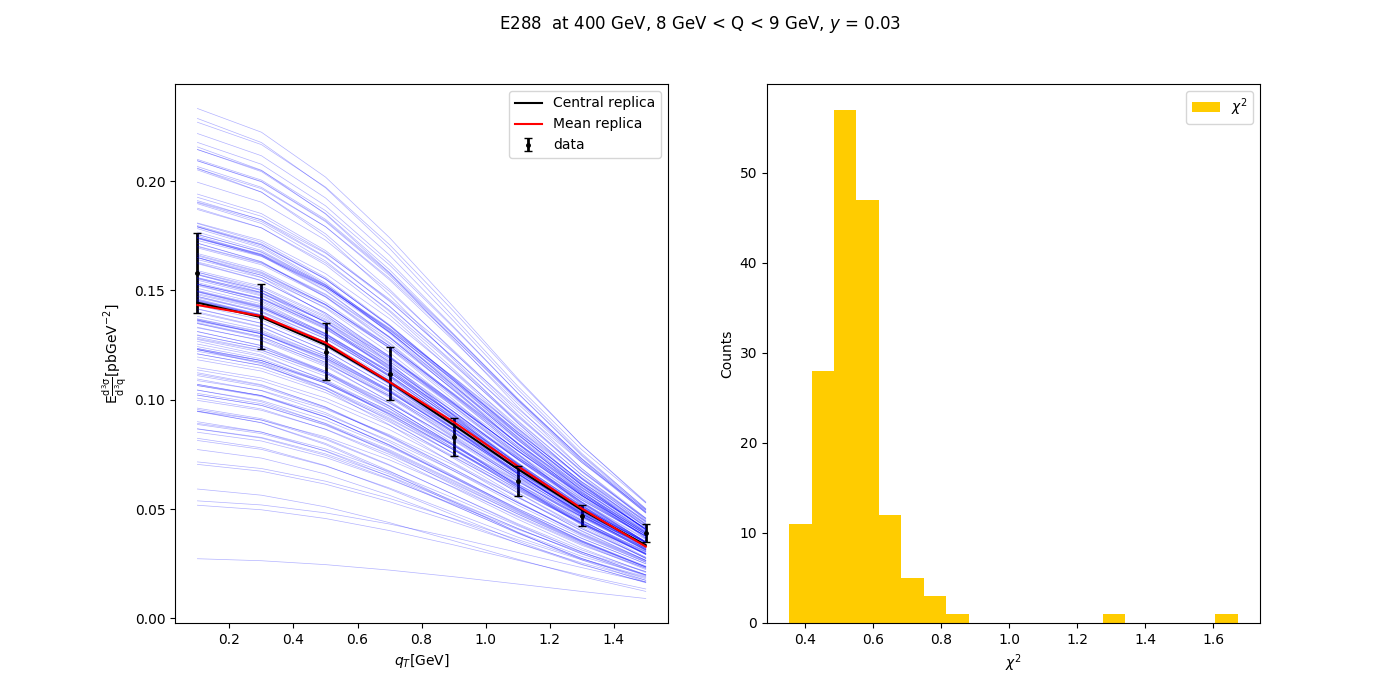
\includegraphics{pngplots/E288_400_Q_8_9.png}
\caption{E288\_400\_Q\_8\_9 data-theory comparison}
\end{figure}

\begin{figure}
\centering
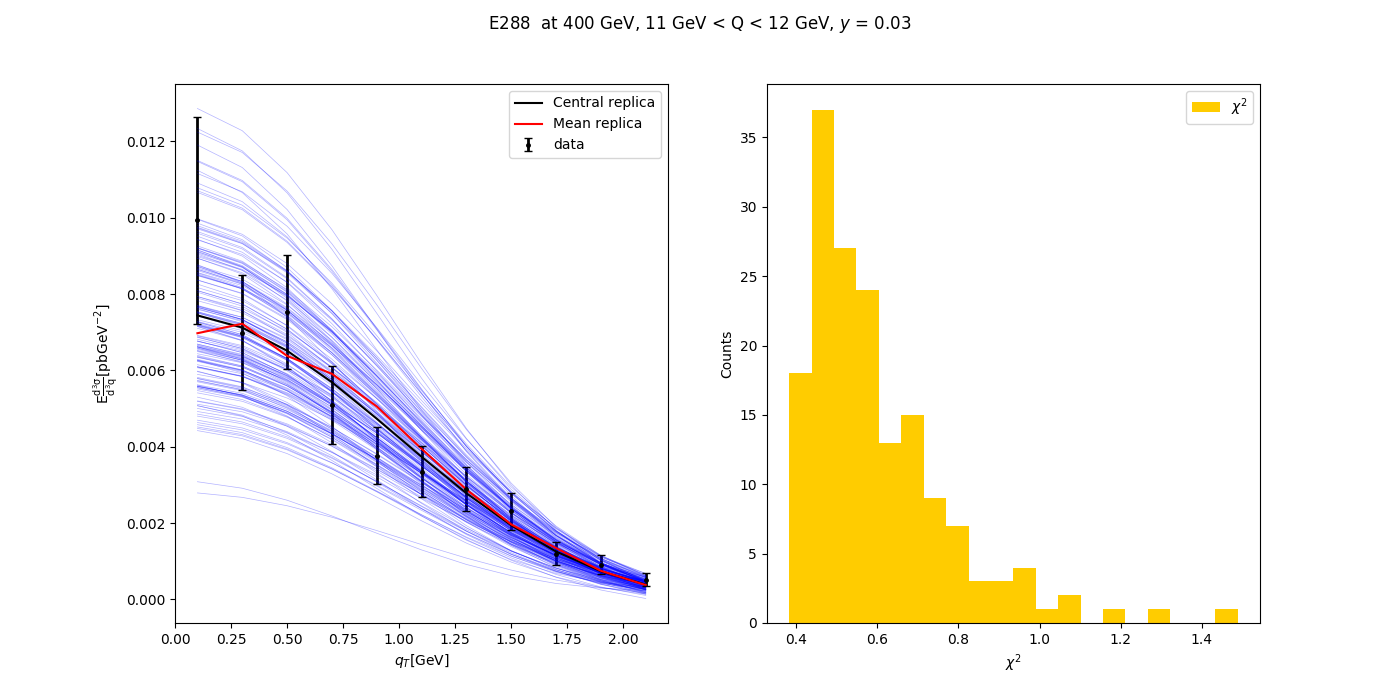
\includegraphics{pngplots/E288_400_Q_11_12.png}
\caption{E288\_400\_Q\_11\_12 data-theory comparison}
\end{figure}

\begin{figure}
\centering
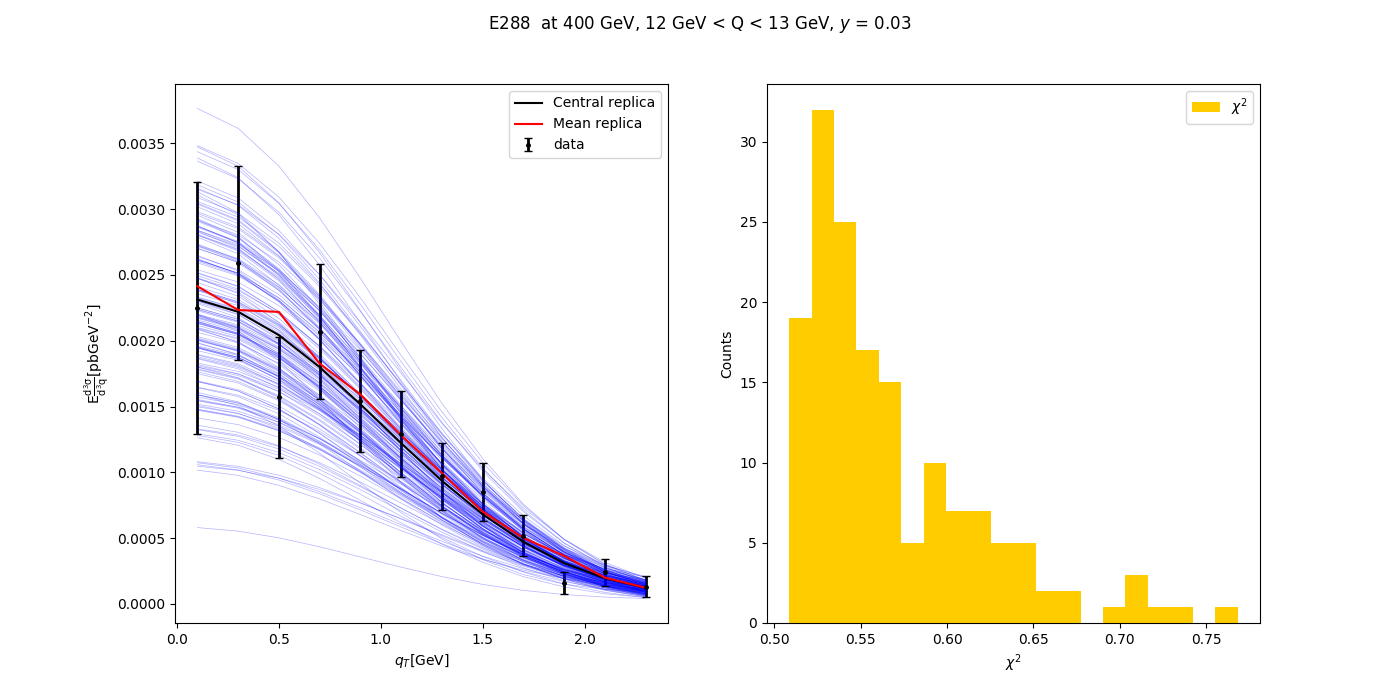
\includegraphics{pngplots/E288_400_Q_12_13.png}
\caption{E288\_400\_Q\_12\_13 data-theory comparison}
\end{figure}

\begin{figure}
\centering
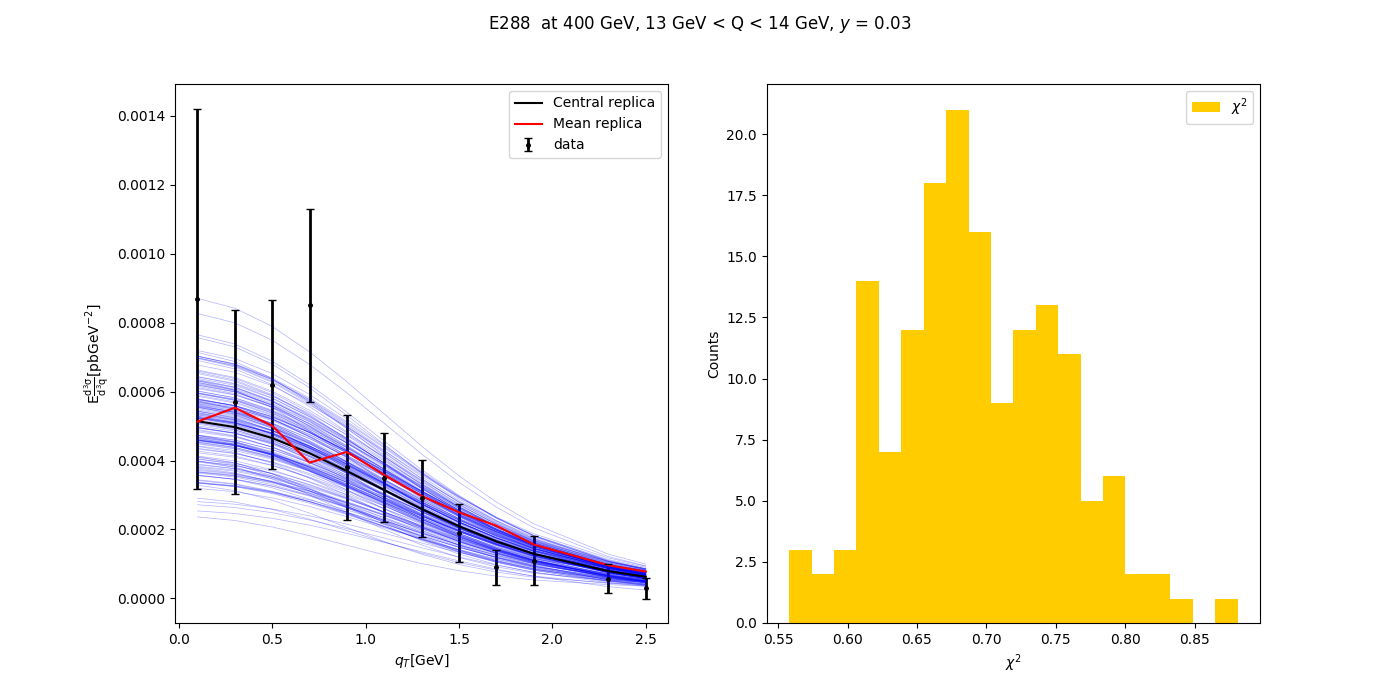
\includegraphics{pngplots/E288_400_Q_13_14.png}
\caption{E288\_400\_Q\_13\_14 data-theory comparison}
\end{figure}

\begin{figure}
\centering
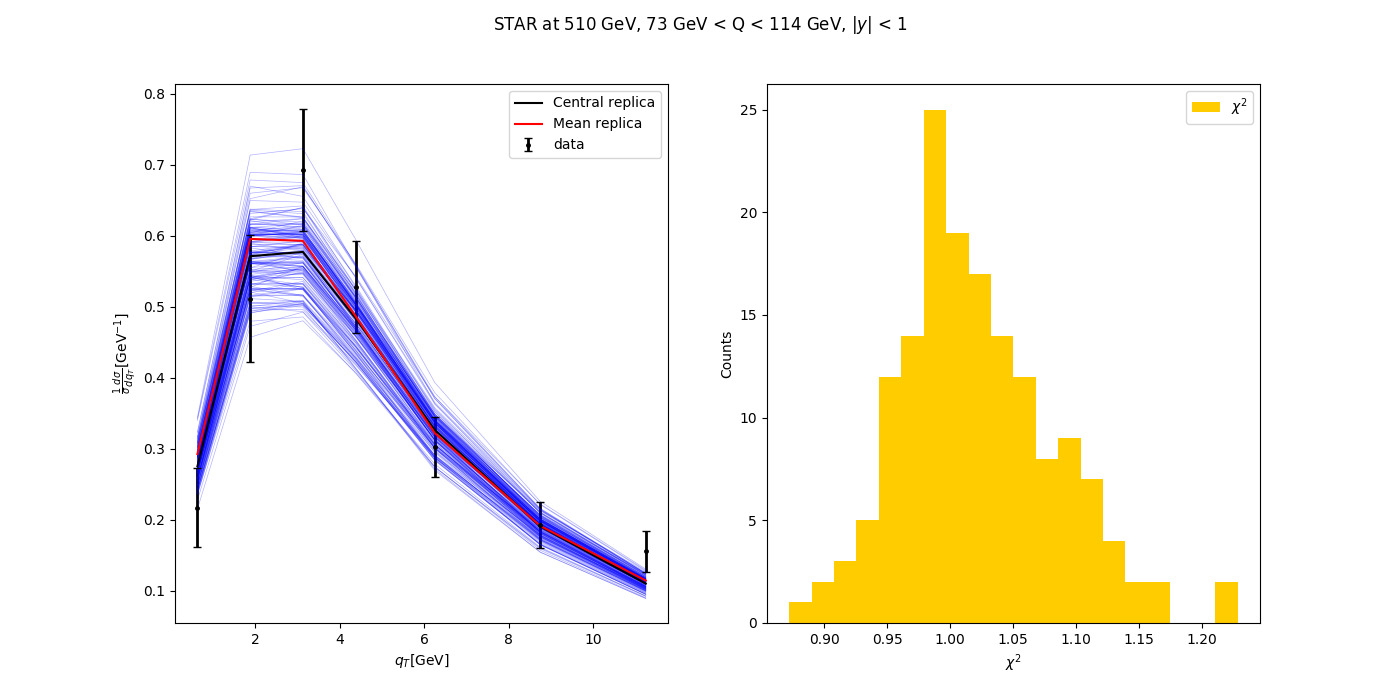
\includegraphics{pngplots/STAR_510.png}
\caption{STAR\_510 data-theory comparison}
\end{figure}

\begin{figure}
\centering
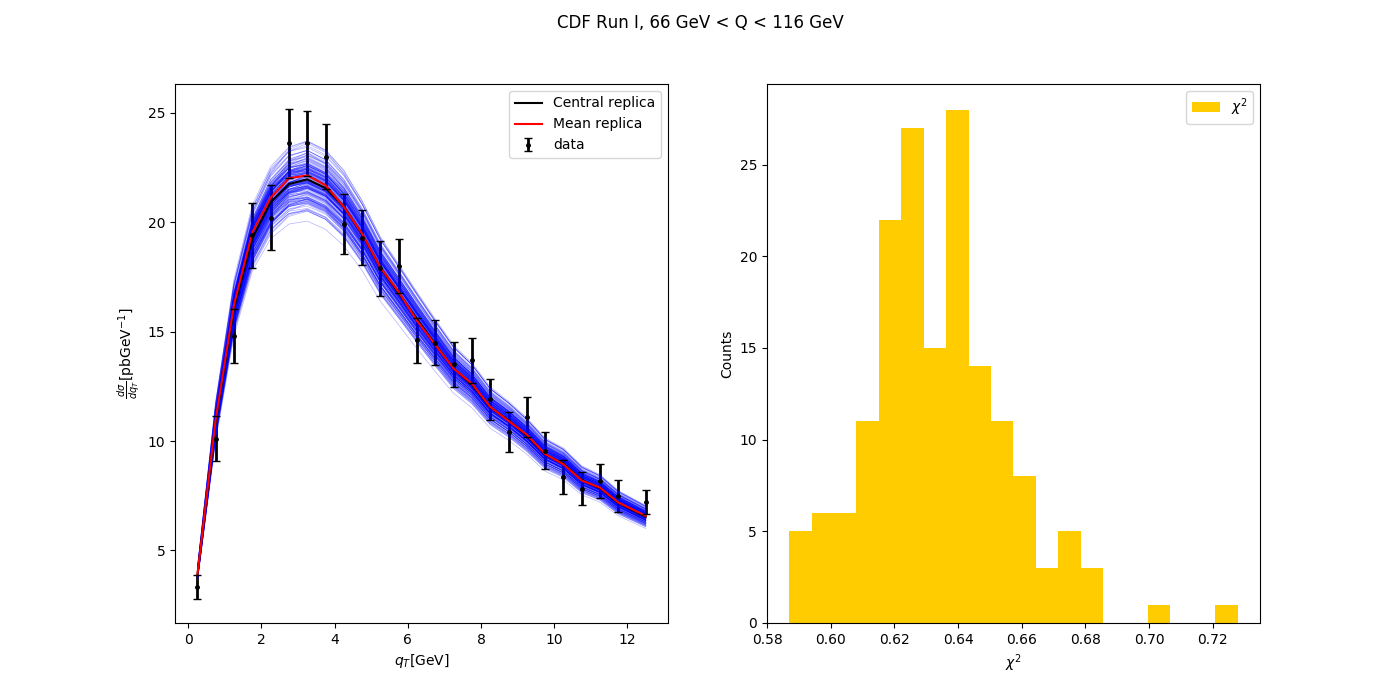
\includegraphics{pngplots/CDF_RunI.png}
\caption{CDF\_RunI data-theory comparison}
\end{figure}

\begin{figure}
\centering
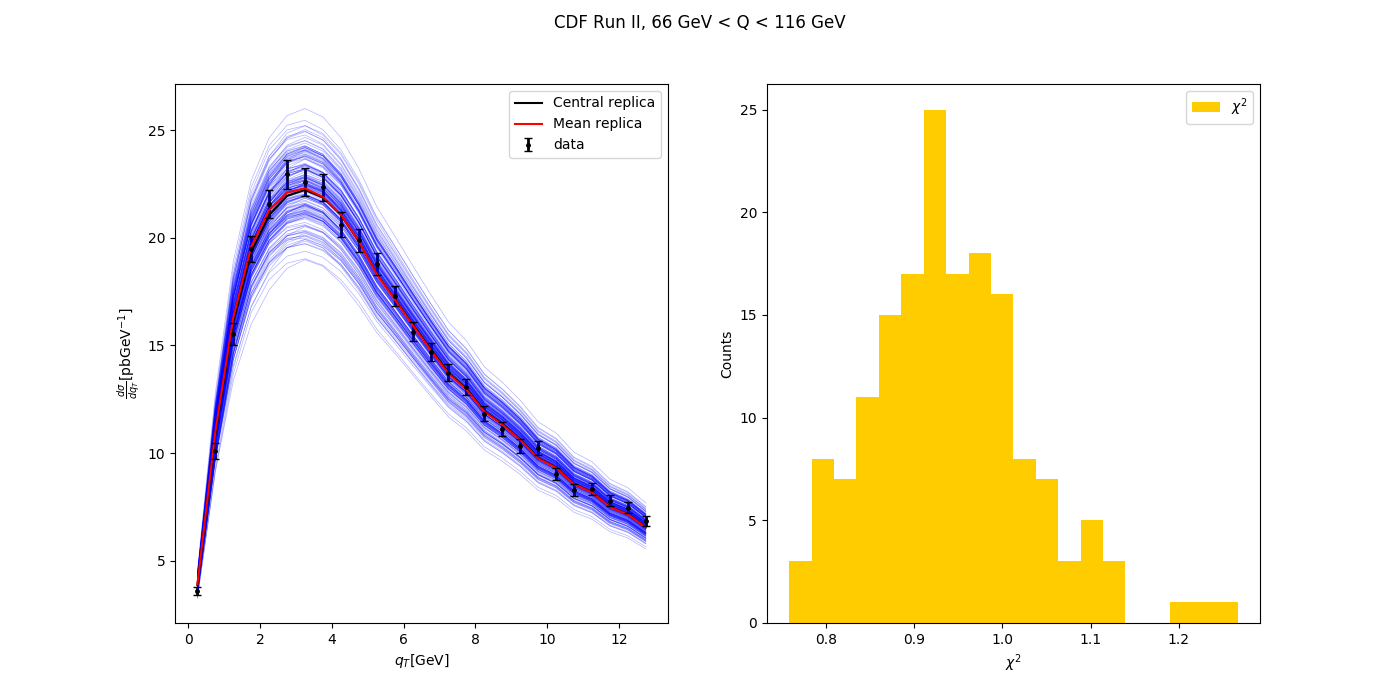
\includegraphics{pngplots/CDF_RunII.png}
\caption{CDF\_RunII data-theory comparison}
\end{figure}

\begin{figure}
\centering
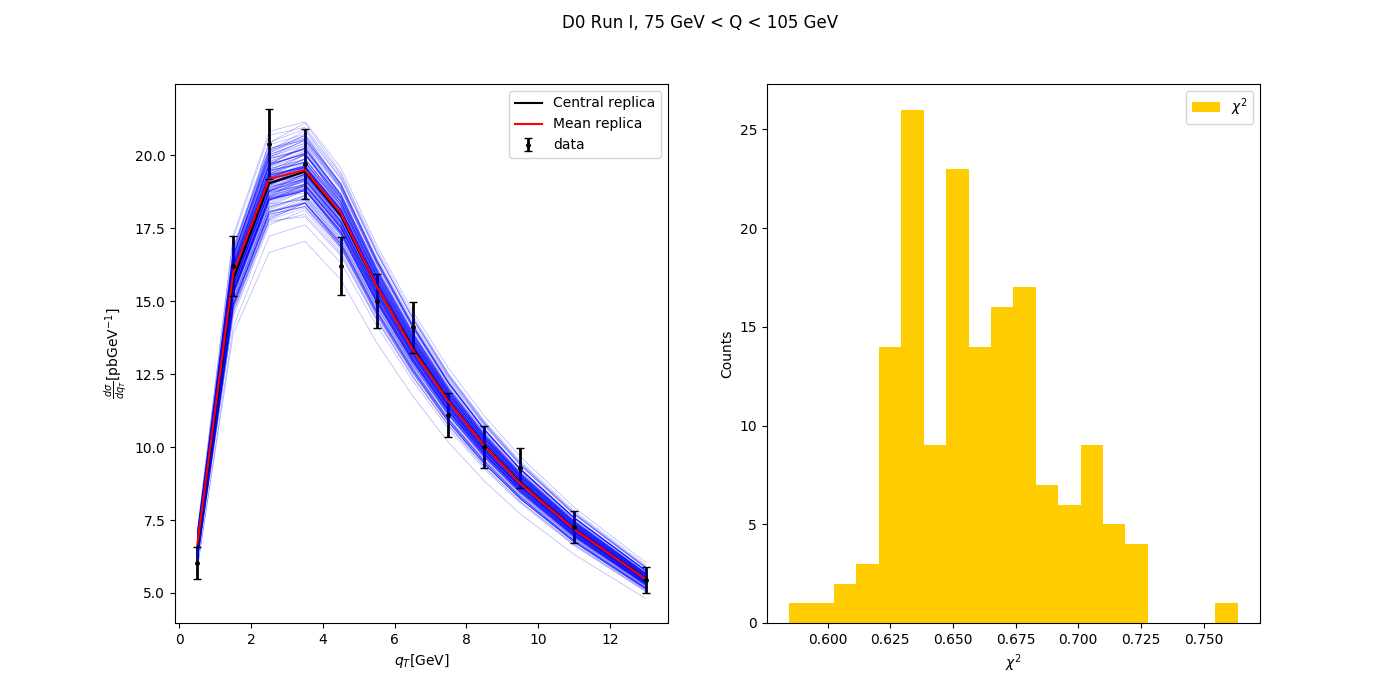
\includegraphics{pngplots/D0_RunI.png}
\caption{D0\_RunI data-theory comparison}
\end{figure}

\begin{figure}
\centering
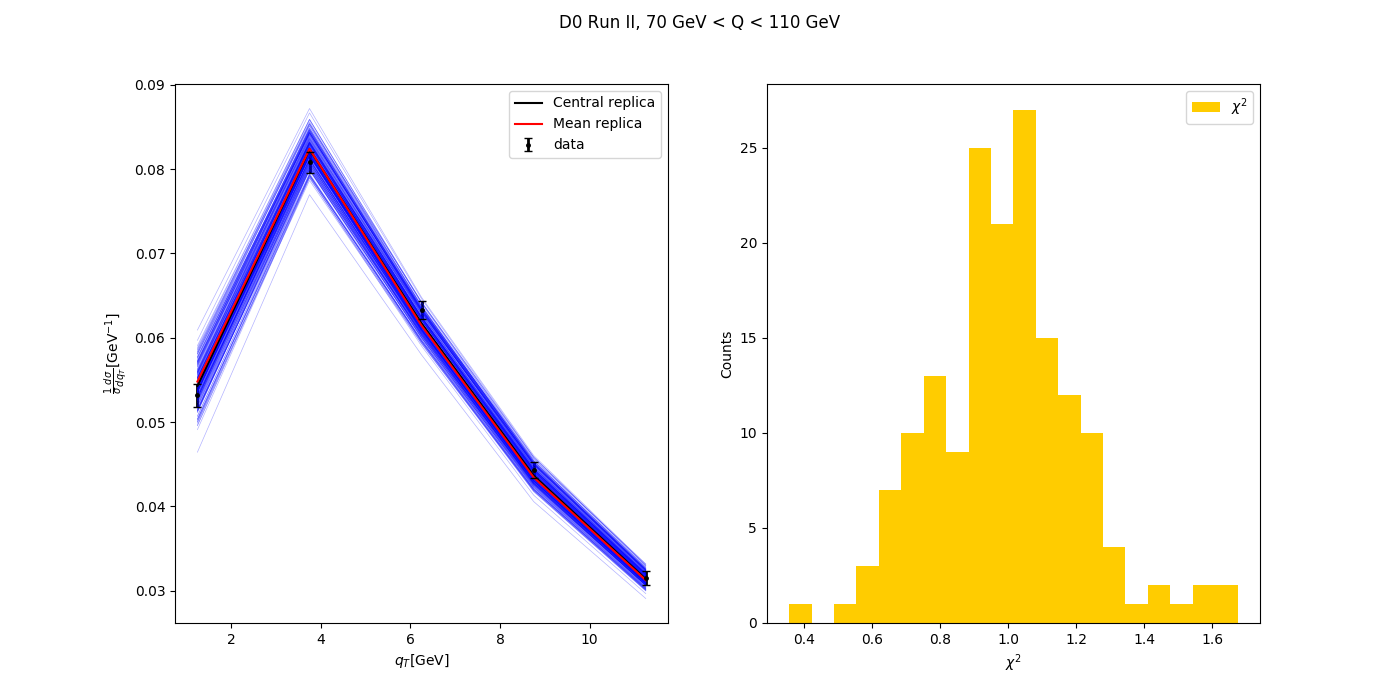
\includegraphics{pngplots/D0_RunII.png}
\caption{D0\_RunII data-theory comparison}
\end{figure}

\begin{figure}
\centering
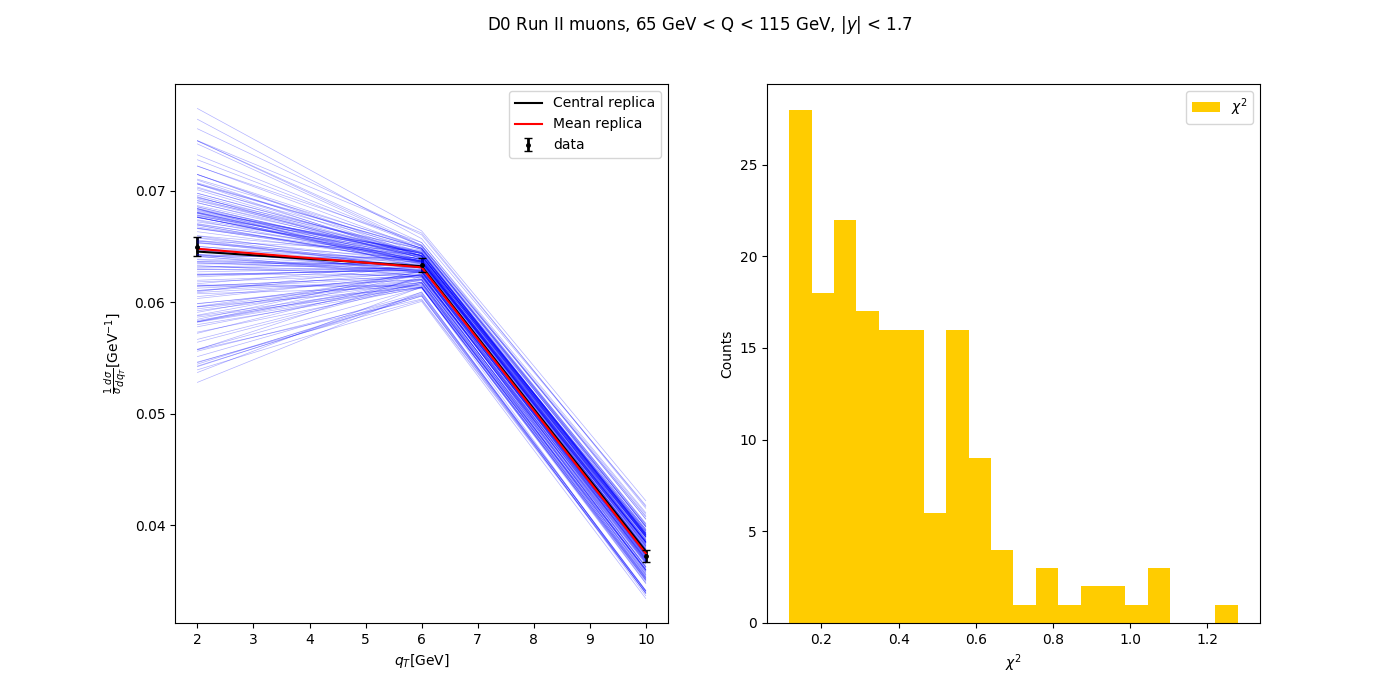
\includegraphics{pngplots/D0_RunIImu.png}
\caption{D0\_RunIImu data-theory comparison}
\end{figure}

\begin{figure}
\centering
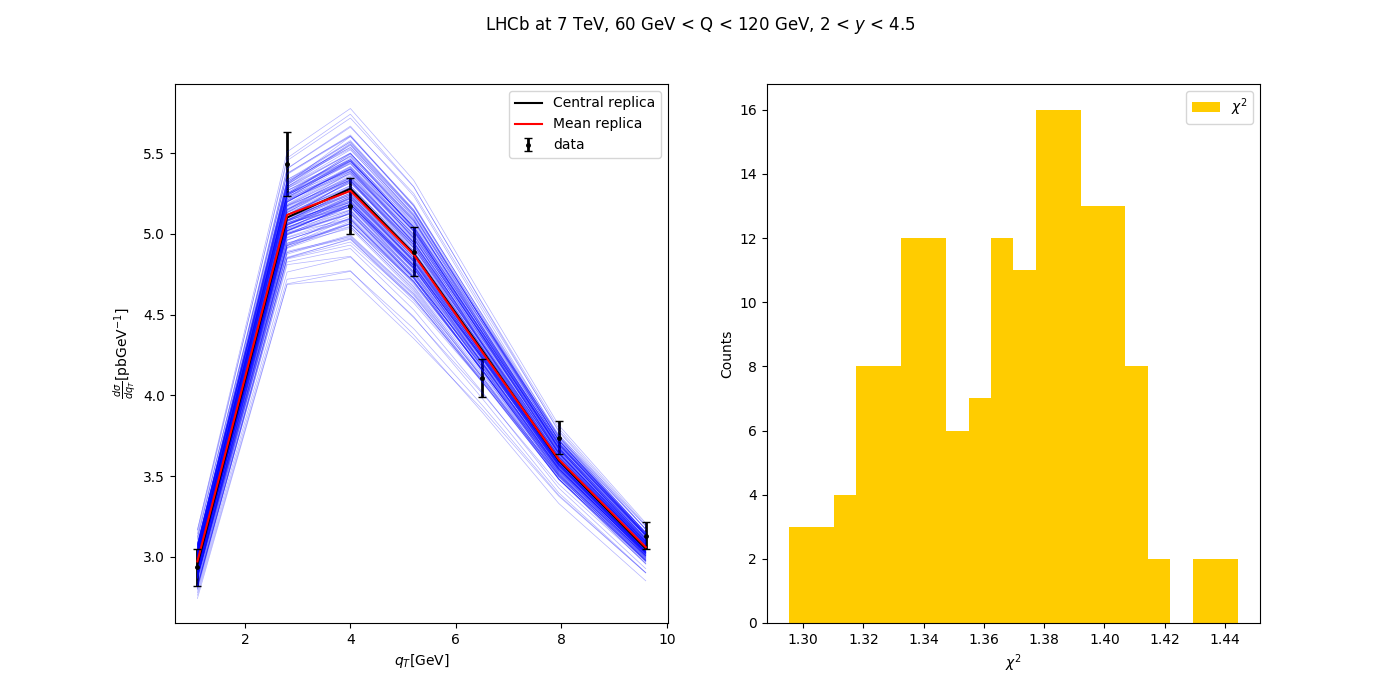
\includegraphics{pngplots/LHCb_7TeV.png}
\caption{LHCb\_7TeV data-theory comparison}
\end{figure}

\begin{figure}
\centering
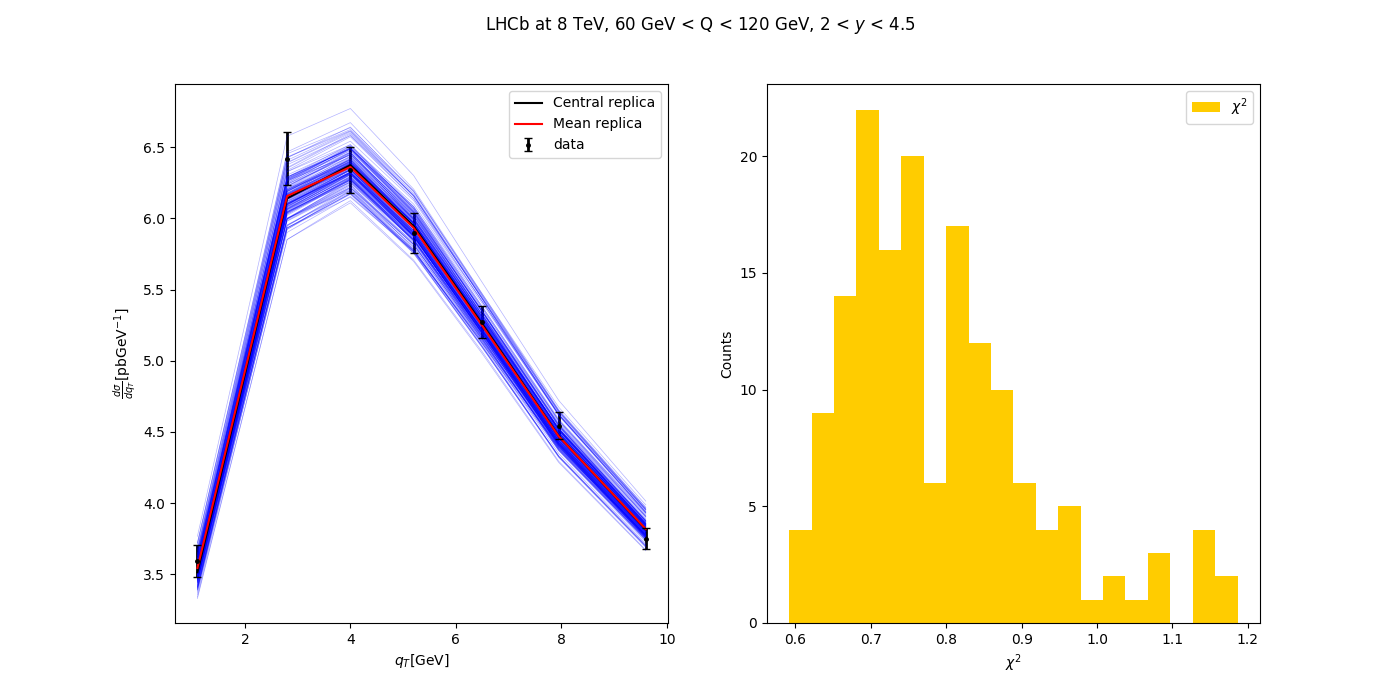
\includegraphics{pngplots/LHCb_8TeV.png}
\caption{LHCb\_8TeV data-theory comparison}
\end{figure}

\begin{figure}
\centering
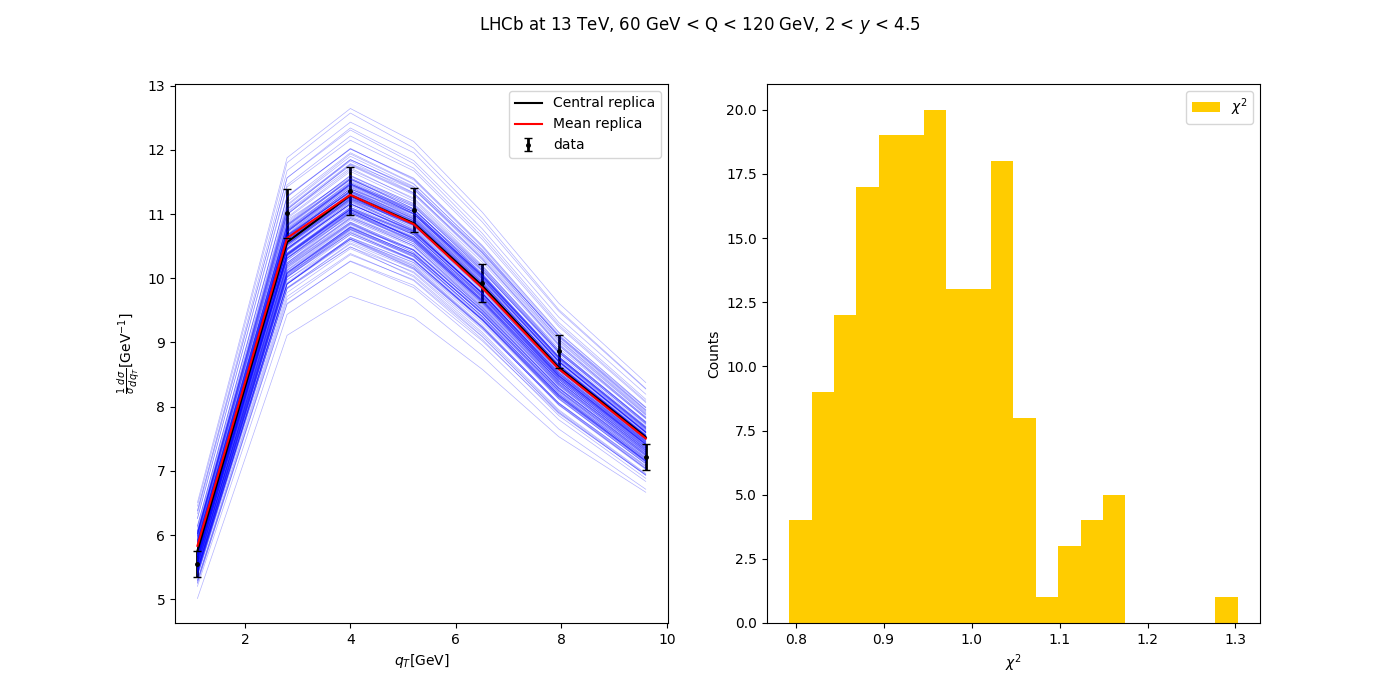
\includegraphics{pngplots/LHCb_13TeV.png}
\caption{LHCb\_13TeV data-theory comparison}
\end{figure}

\begin{figure}
\centering
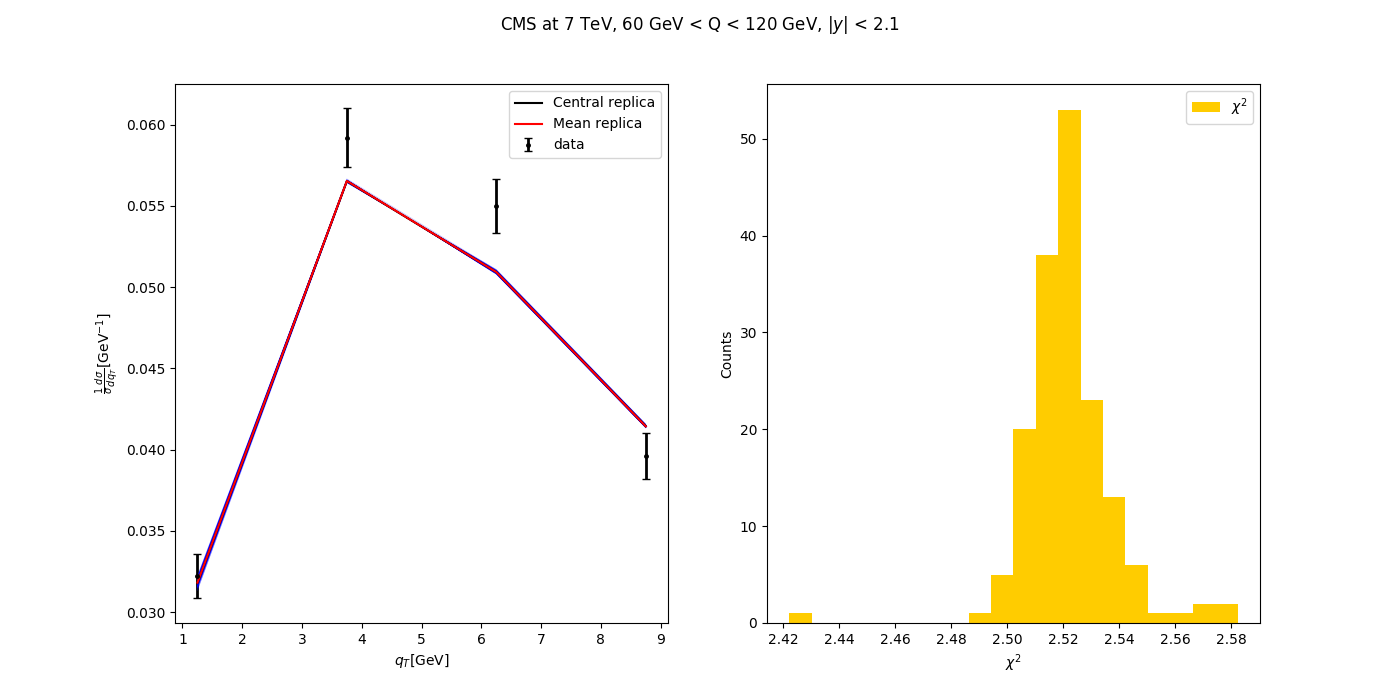
\includegraphics{pngplots/CMS_7TeV.png}
\caption{CMS\_7TeV data-theory comparison}
\end{figure}

\begin{figure}
\centering
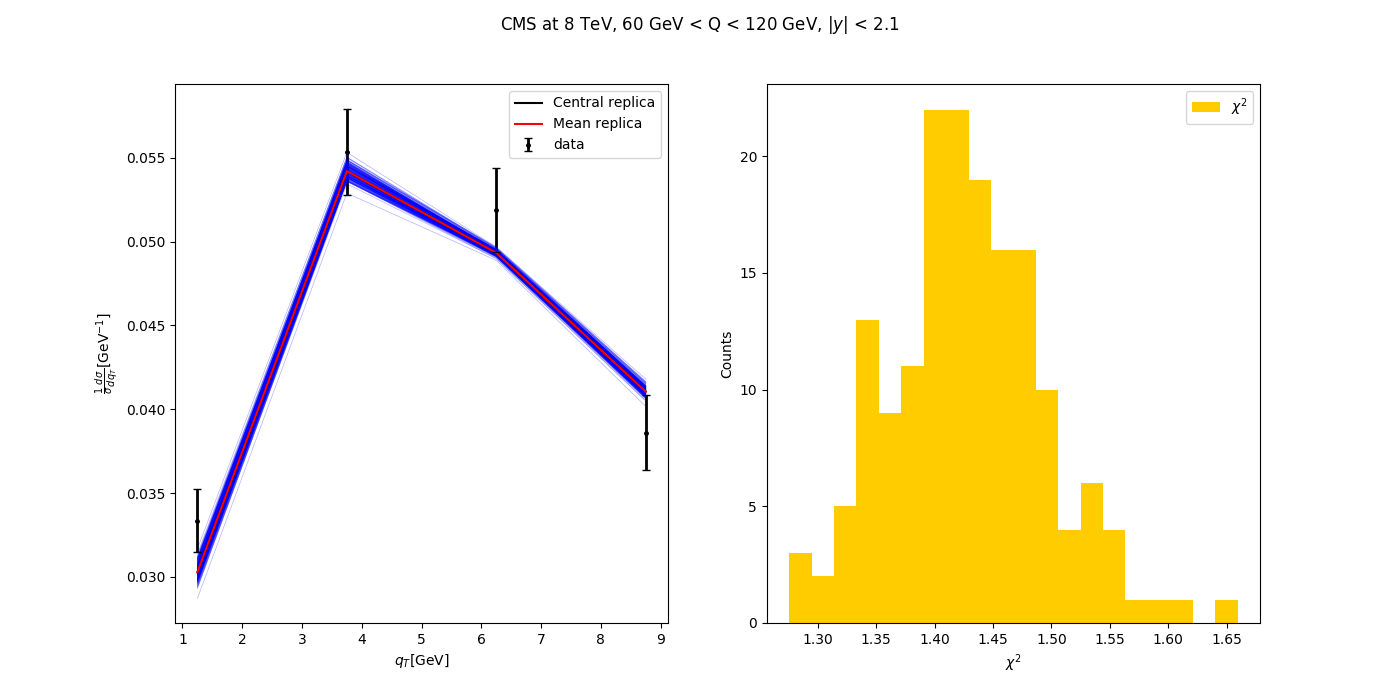
\includegraphics{pngplots/CMS_8TeV.png}
\caption{CMS\_8TeV data-theory comparison}
\end{figure}

\begin{figure}
\centering
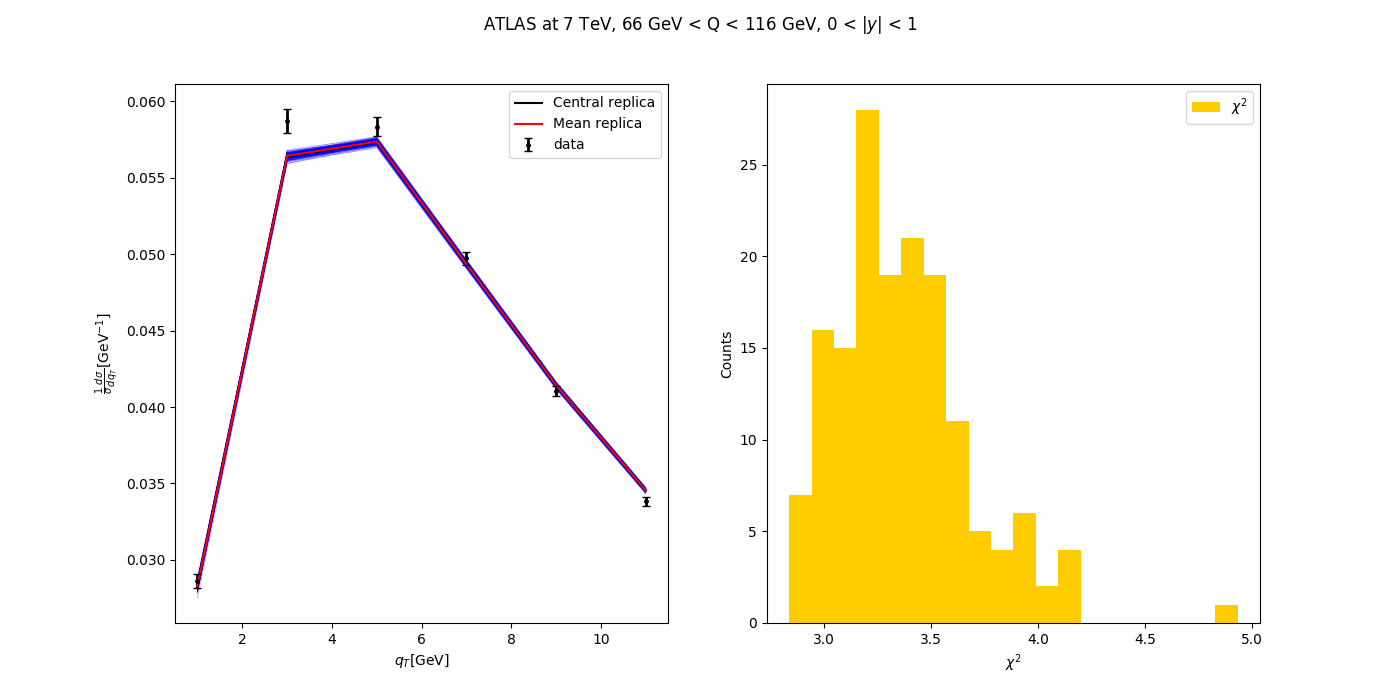
\includegraphics{pngplots/ATLAS_7TeV_y_0_1.png}
\caption{ATLAS\_7TeV\_y\_0\_1 data-theory comparison}
\end{figure}

\begin{figure}
\centering
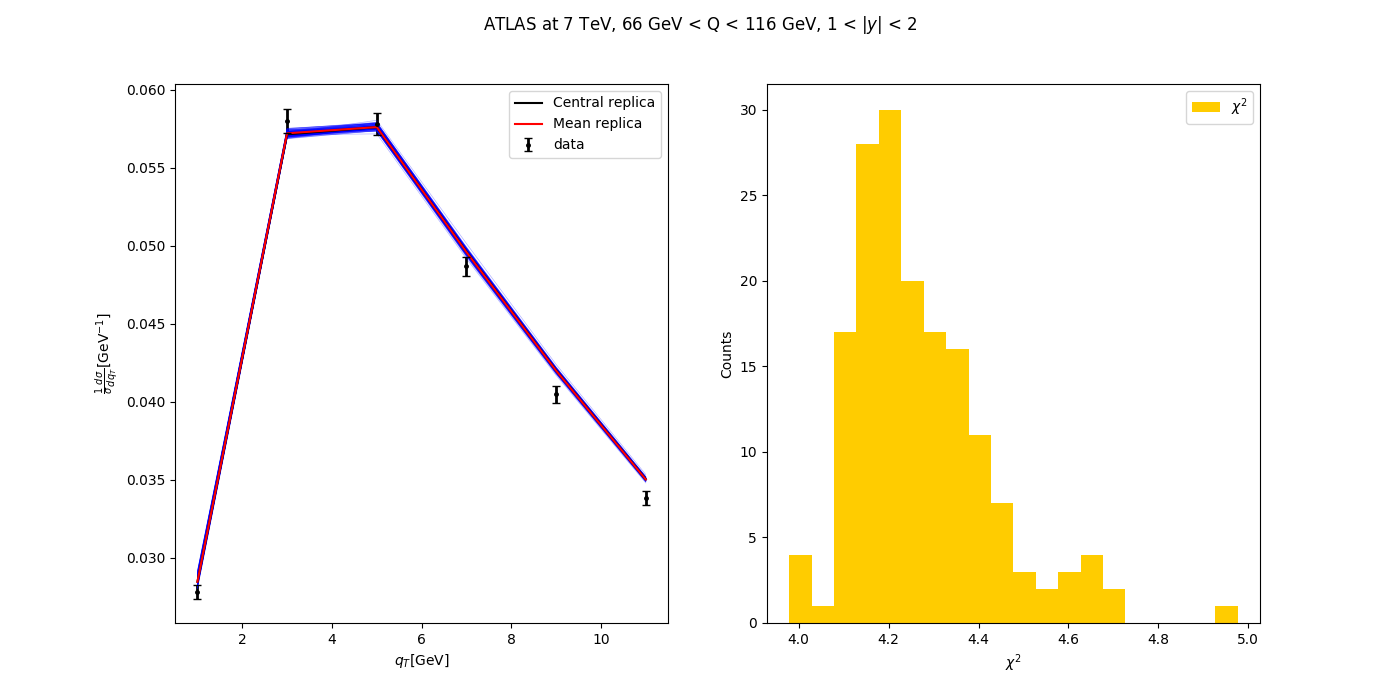
\includegraphics{pngplots/ATLAS_7TeV_y_1_2.png}
\caption{ATLAS\_7TeV\_y\_1\_2 data-theory comparison}
\end{figure}

\begin{figure}
\centering
\includegraphics{pngplots/ATLAS_7TeV_y_2_2.4.png}
\caption{ATLAS\_7TeV\_y\_2\_2.4 data-theory comparison}
\end{figure}

\begin{figure}
\centering
\includegraphics{pngplots/ATLAS_8TeV_y_0_0.4.png}
\caption{ATLAS\_8TeV\_y\_0\_0.4 data-theory comparison}
\end{figure}

\begin{figure}
\centering
\includegraphics{pngplots/ATLAS_8TeV_y_0.4_0.8.png}
\caption{ATLAS\_8TeV\_y\_0.4\_0.8 data-theory comparison}
\end{figure}

\begin{figure}
\centering
\includegraphics{pngplots/ATLAS_8TeV_y_0.8_1.2.png}
\caption{ATLAS\_8TeV\_y\_0.8\_1.2 data-theory comparison}
\end{figure}

\begin{figure}
\centering
\includegraphics{pngplots/ATLAS_8TeV_y_1.2_1.6.png}
\caption{ATLAS\_8TeV\_y\_1.2\_1.6 data-theory comparison}
\end{figure}

\begin{figure}
\centering
\includegraphics{pngplots/ATLAS_8TeV_y_1.6_2.png}
\caption{ATLAS\_8TeV\_y\_1.6\_2 data-theory comparison}
\end{figure}

\begin{figure}
\centering
\includegraphics{pngplots/ATLAS_8TeV_y_2_2.4.png}
\caption{ATLAS\_8TeV\_y\_2\_2.4 data-theory comparison}
\end{figure}

\begin{figure}
\centering
\includegraphics{pngplots/ATLAS_8TeV_Q_46_66.png}
\caption{ATLAS\_8TeV\_Q\_46\_66 data-theory comparison}
\end{figure}

\begin{figure}
\centering
\includegraphics{pngplots/ATLAS_8TeV_Q_116_150.png}
\caption{ATLAS\_8TeV\_Q\_116\_150 data-theory comparison}
\end{figure}

\end{document}
